% !TEX program = xelatex
\documentclass[UTF8,a4paper,12pt]{ctexart}
\usepackage{geometry}
\geometry{left=2.3cm,right=2.3cm,top=2.5cm,bottom=2.5cm}
\usepackage{amsmath,amssymb,bm}
\usepackage{graphicx}
\usepackage{booktabs,array,multirow}
\usepackage{subcaption}
\usepackage{enumitem}
\usepackage{float}
\usepackage{hyperref}
\hypersetup{hidelinks}
\graphicspath{{exp5_images/}}
\newcommand{\blank}[1][2.5cm]{\mbox{\underline{\hspace{#1}}}}
\newcommand{\answer}{\par\noindent\textbf{填写：}\blank[0.86\textwidth]\par}
\numberwithin{equation}{section}

\title{《风力机叶片模型的模态分析》实验报告}
\author{姓名\blank[2.5cm] \quad 学号\blank[3cm] \quad 同组成员\blank[4cm]\\[1em]
实验地点\blank[3cm] \quad 实验日期\blank[4cm]}
\date{}
\begin{document}
\maketitle
\tableofcontents
\clearpage

\section{实验目的}
\begin{enumerate}
  \item 了解激光测振仪的工作原理和使用方法。
  \item 掌握激励器激振法及其特点。
  \item 掌握激振器激振、激光测振仪拾振的频响函数测试方法及测试技术。
  \item 掌握多自由度系统的固有频率、主振型、阻尼率等结构模态参数的识别方法。
\end{enumerate}

\section{实验装置、仪器及器材}
\begin{enumerate}
  \item 单点激光测振仪（Polttec，OFV-3001）。
  \item 激光发射器（Polttec GmbH，OFV-353）。
  \item 激振器（Mini Shaker Type 4810）。
  \item 函数/任意波形发生器（RIGOL，DG5072，70 MHz，1 GSa/s）。
  \item 电荷放大器（HY1432，秦皇岛海鹰科技开发有限公司）。
  \item 功率放大器（Bruel \& Kjaer，Power Amplifier，Type 2706）。
  \item USB 口多功能采集模块。
  \item 力传感器（CL-YD-312 20523）。
  \item 风力机叶片模型（上贴反光条）。
  \item 计算机（ThinkPad）。
  \item 钢尺（100 cm，北京五金工具十厂）。
  \item 导线若干。
\end{enumerate}

\section{实验内容}
用激光测振仪测得 Periodic Chirp 周期线性调频脉冲激励信号与 Pseudo Random 伪随机激励信号作用下的响应，对信号做 FFT 变换并求频响函数，得到风力机叶片模型的固有频率、振型、阻尼率，进行分析与讨论。

\section{实验原理与测量过程}
\subsection{实验原理}
振动表征一种运动的物理量作时而增大、时而减小的反复变化。从运动学观点看，它是某些物理量（位移、速度、加速度）在某一数值附近随时间的变化关系。振动理论可用于响应分析，通过激励和系统特性得出系统响应，为结构强度设计提供依据；也可用于系统识别，通过激励和响应识别系统特性参数；还可用于环境预测，通过系统特性和响应确定激励，识别系统环境的振动特性。系统特性参数一般为结构模态参数，包括固有频率 $\omega$、固有振型 $\{\varphi_i\}$、阻尼率 $\zeta_i$ 等。

对于多自由度系统，有动力学方程
\begin{equation}
  [M]\{\ddot{x}\}+[c]\{\dot{x}\}+[k]\{x\}=\{f(t)\}.
  \label{eq:exp5-dynamics}
\end{equation}
对于无阻尼自由振动，方程退化为
\begin{equation}
  [M]\{\ddot{x}\}+[k]\{x\}=0.
  \label{eq:exp5-free}
\end{equation}
设结构固有频率为 $\omega$，固有振型为 $\{\varphi_i\}$，则 $\{x\}=\{\varphi_i\}\sin(\omega t+\psi)$ 必然是上式的一个解。代入有
\begin{equation}
  ([k]-\omega^2[M])\{\varphi\}=\{0\}.
\end{equation}
若有非零解，则 $|[k]-\omega^2[M]|=0$，解出的特征值 $\omega_j$ 即为第 $j$ 阶固有频率；由 $([k]-\omega_j^2[M])\{\varphi_j\}=\{0\}$ 解出的特征向量 $\{\varphi_j\}$ 即为对应固有振型。方程\eqref{eq:exp5-free}的通解为
\begin{equation}
  \{x\}=\sum_{j=1}^{n}\{\varphi_j\}\sin(\omega_jt+\psi_j).
\end{equation}
对方程\eqref{eq:exp5-dynamics}做傅里叶变换可得
\begin{equation}
  (-\omega^2[M]+i\omega[c]+[k])\{X(\omega)\}=\{F(\omega)\}.
\end{equation}
对应的位移频响函数为
\begin{equation}
  H_{ij}(\omega)=\frac{X_i(\omega)}{F_j(\omega)}
  =\sum_{k=1}^{n}\frac{\varphi_{ik}\varphi_{jk}}
  {m_k(\omega_k^2-\omega^2+2i\zeta_k\omega\omega_k)}.
\end{equation}
系统的总频率响应函数为各阶模态频率响应函数之和。由于速度为位移对时间的导数，因此速度频响函数为
\begin{equation}
  H^v_{ij}(\omega)=\frac{\dot{X}_i(\omega)}{F_j(\omega)}=i\omega H_{ij}(\omega).
\end{equation}

对于单自由度系统的速度频响函数，可以得到图\ref{fig:exp5-frf-curves}所示曲线。对于多自由度系统，当模态不密集时，可根据速度频响函数的实频曲线（图\ref{fig:exp5-real-frf}）由峰值 $p_k$ 处的频率得到对应的固有频率 $\omega_k$。

\begin{figure}[H]
  \centering
  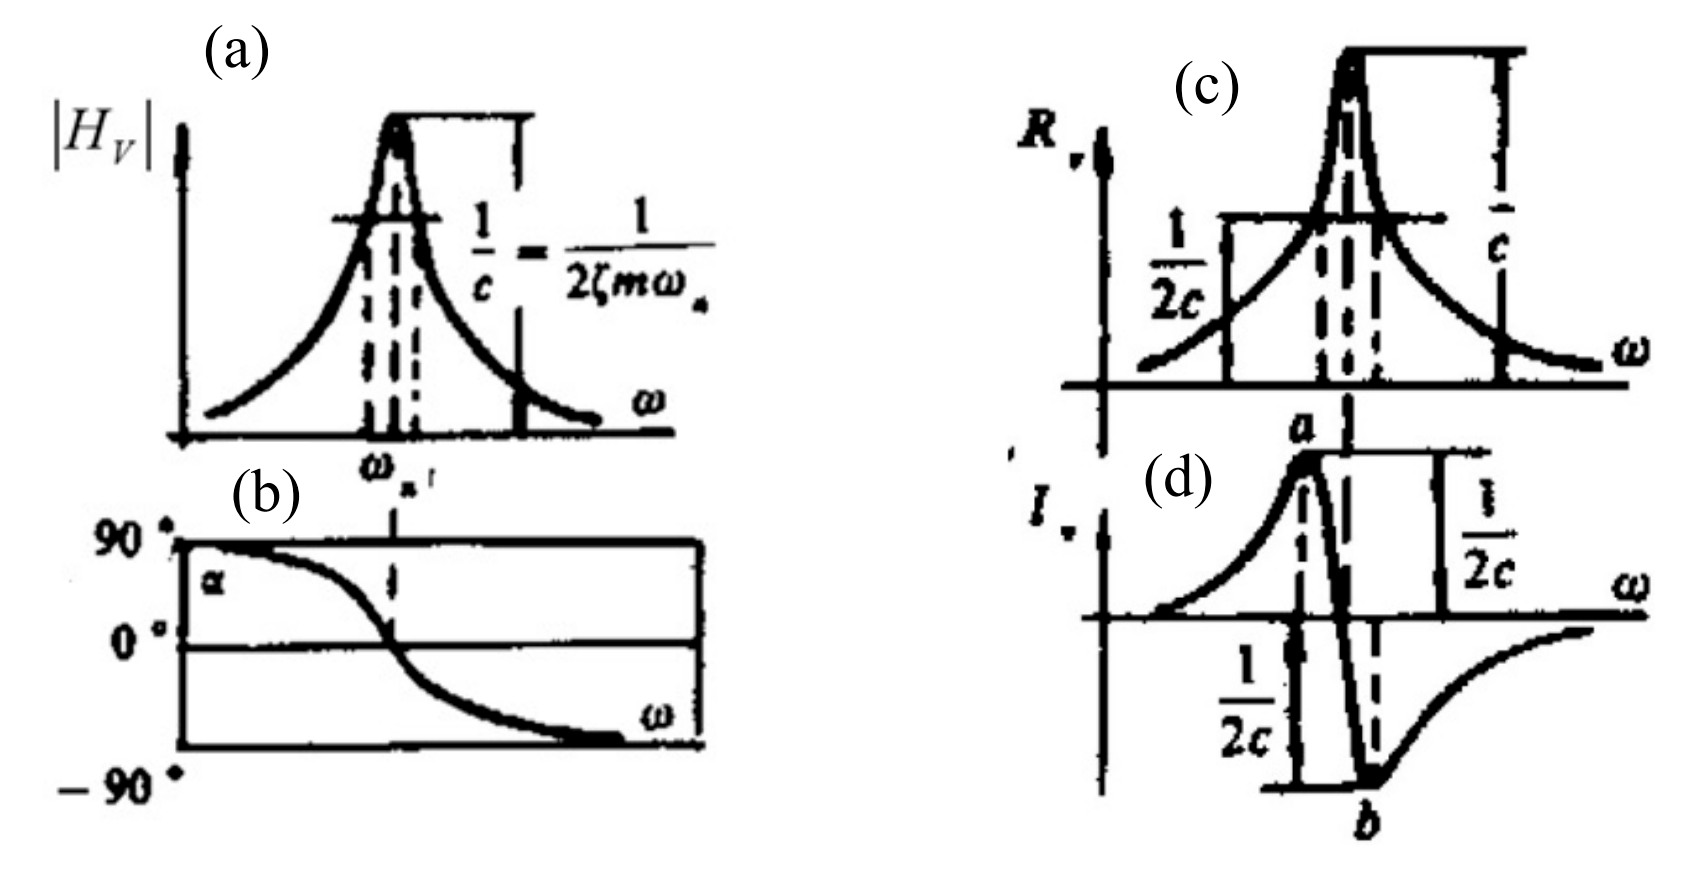
\includegraphics[width=0.82\textwidth]{p04_img01.png}
  \caption{速度频响函数图：(a) 幅频曲线；(b) 相频曲线；(c) 实频曲线；(d) 虚频曲线}
  \label{fig:exp5-frf-curves}
\end{figure}

\begin{figure}[H]
  \centering
  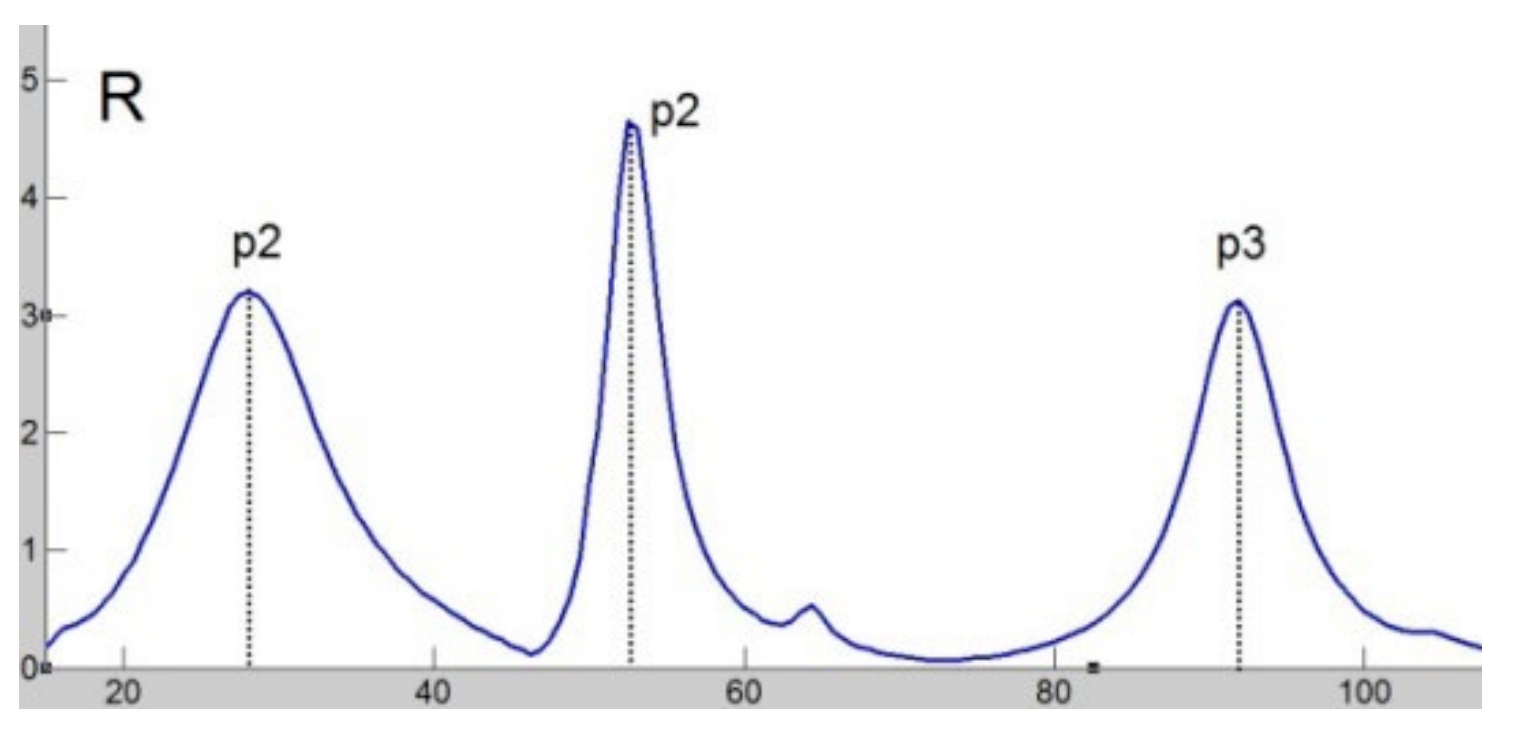
\includegraphics[width=0.52\textwidth]{p04_img02.png}
  \caption{实频曲线示意图}
  \label{fig:exp5-real-frf}
\end{figure}

单阶模态对速度频响函数的贡献及其实部可写为
\begin{align}
  H^v_{ij}(\omega)&=\frac{i\omega\varphi_{ik}\varphi_{jk}}
  {m_k(\omega_k^2-\omega^2+2i\zeta_k\omega\omega_k)},\\
  \operatorname{Re}H^v_{ij}(\omega)&=
  \frac{2\zeta_k\omega_k\omega^2\varphi_{ik}\varphi_{jk}}
  {m_k\left[(\omega_k^2-\omega^2)^2+4\zeta_k^2\omega^2\omega_k^2\right]}.
\end{align}
令 $A_{ij}^k=\varphi_{ik}\varphi_{jk}/m_k$，则
\begin{equation}
  \operatorname{Re}H^v_{ij}(\omega)=
  \frac{2\zeta_k\omega_k\omega^2A_{ij}^k}
  {(\omega_k^2-\omega^2)^2+4\zeta_k^2\omega^2\omega_k^2}.
\end{equation}
当 $\omega=\omega_k$ 时，
\begin{equation}
  A_{ij}^k=2\zeta_k\omega_k\operatorname{Re}H^v_{ij}(\omega_k).
\end{equation}
可设 $m_k=1$，则 $\varphi_{ik}=A_{ij}^k/\varphi_{jk}$。其中，$A_{ij}^k$ 正比于速度频响函数的实部，$j$ 为激振点（此处为单个激振），$k$ 为共振阶数，$\varphi_{jk}$ 为定值。因此，$k$ 阶固有振型 $\varphi_{ik}$ 为所有测点处实频曲线第 $k$ 个峰值所连成的曲线。

值得指出的是，振动测试往往是一点激励、多点测振，或多点激励、一点测振，且激振点与测振点不同。对于一点激励、多点测振的模态分析，若激振点没有测振，则无法获得激振点处的振型幅值；但仅需要测振点处的振型幅值即可描述振型。因此，在振型分析过程中可令 $\varphi_{jk}=1$（前提是激振点不是振型节点，这在实际振动测试中比较关键）。

针对速度频响函数的实频曲线，可通过半功率点 $a,b$（见图\ref{fig:exp5-half-power}，处于实频曲线峰值的 $1/2$ 处）得到阻尼率
\begin{equation}
  \zeta=\frac{\omega_b-\omega_a}{2\omega_0}.
  \label{eq:exp5-damping}
\end{equation}

\begin{figure}[H]
  \centering
  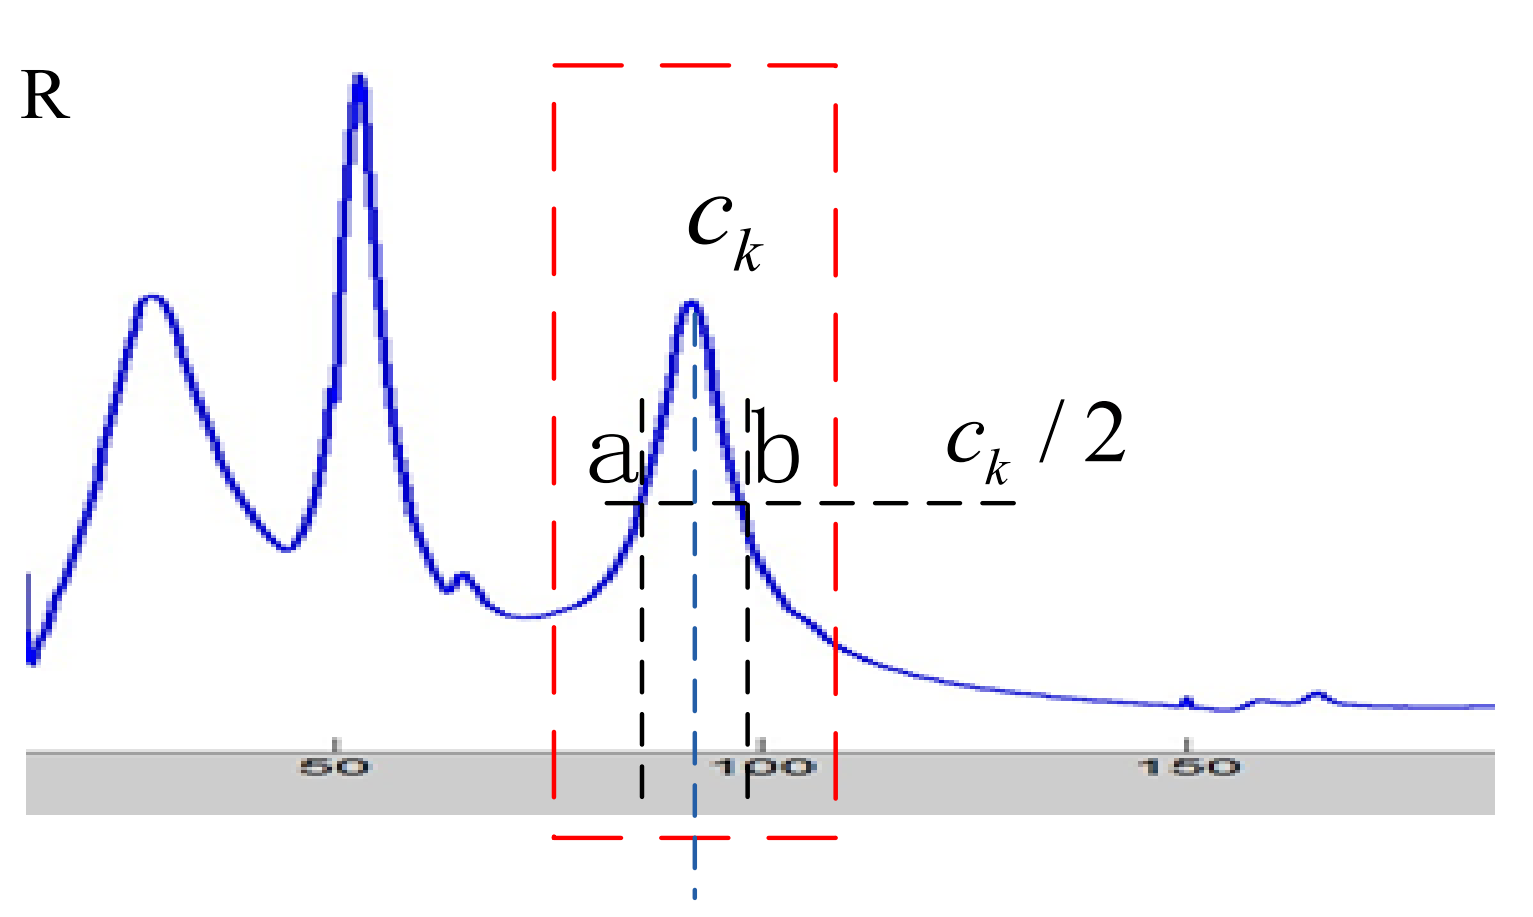
\includegraphics[width=0.5\textwidth]{p05_img01.png}
  \caption{实频曲线的半功率点}
  \label{fig:exp5-half-power}
\end{figure}

对于实验测量过程，激光测振仪发出一束激光照射到振动物体表面，利用多普勒效应，从反射激光的频率得到被测点的运动速度，并可根据速度积分或求导获得位移或加速度。本试验通过激励器激振法进行振动测试。计算机控制输出特定激励信号，通过功率放大器输入激振器，激振器给予模型单点激励；同时激光测振仪通过扫描结构测点获得各测点的振动速度响应信号。经过分析激励信号和速度响应信号，可以获得频率响应函数和结构振动模态参数。实验测试装置如图\ref{fig:exp5-system}所示。

\begin{figure}[H]
  \centering
  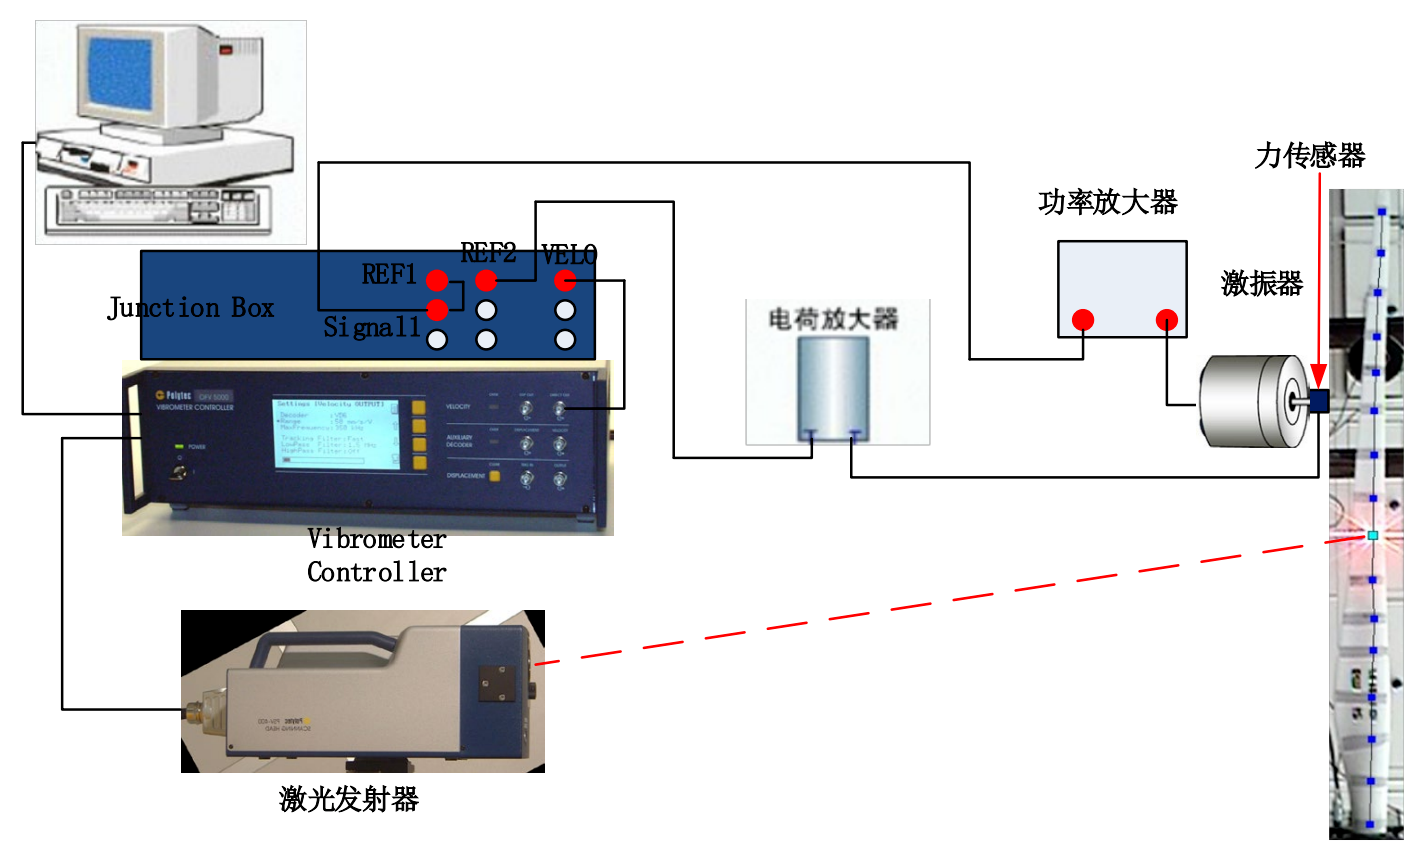
\includegraphics[width=0.7\textwidth]{p05_img02.png}
  \caption{实验装置示意图}
  \label{fig:exp5-system}
\end{figure}

激振器激励信号有以下两种：
\begin{enumerate}[label=\alph*)]
  \item Periodic Chirp 周期线性调频脉冲激励信号：信号载频在给定时间间隔内线性增大或减小，使发射信号的频谱占据一个带宽范围，如图\ref{fig:exp5-chirp}所示。
  \item Pseudo Random 伪随机激励信号：信号在周期 $T$ 内具有随机性，而大于一个周期则显示非随机性。伪随机激励信号具有快速、可变焦、无波漏，以及良好的波峰因子和信噪比，如图\ref{fig:exp5-random}所示。
\end{enumerate}

\begin{figure}[H]
  \centering
  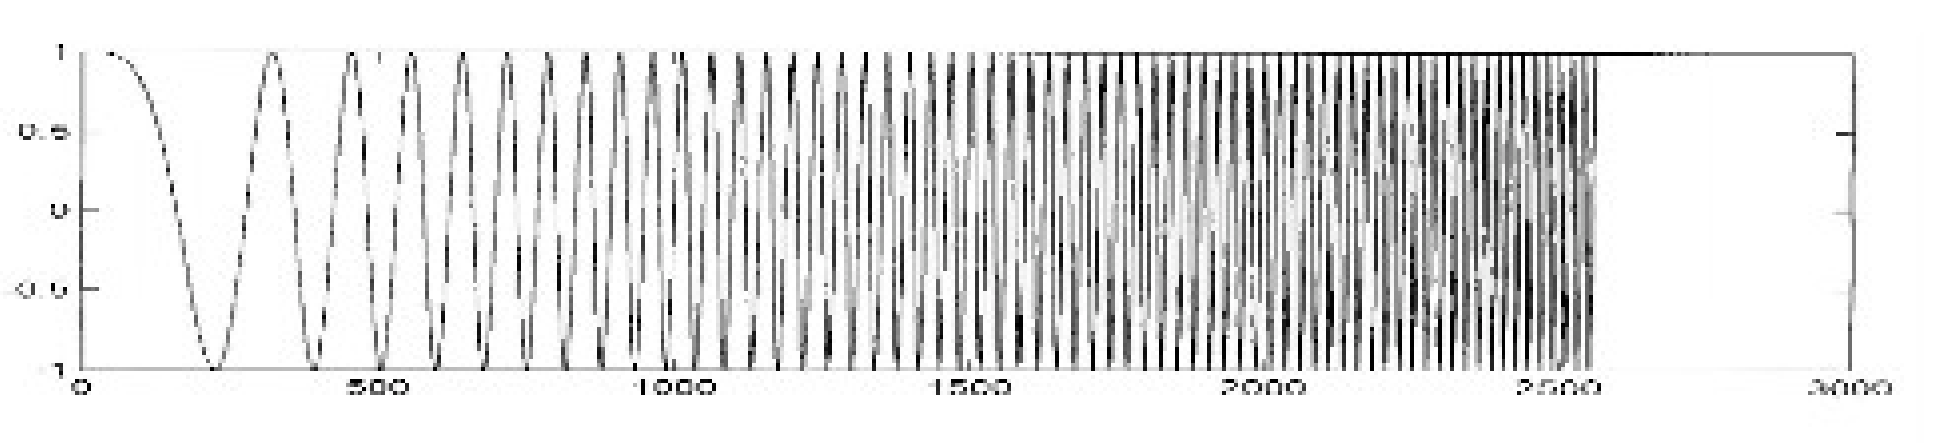
\includegraphics[width=0.65\textwidth]{p05_img03.png}
  \caption{Periodic Chirp 周期线性调频脉冲激励信号}
  \label{fig:exp5-chirp}
\end{figure}

\begin{figure}[H]
  \centering
  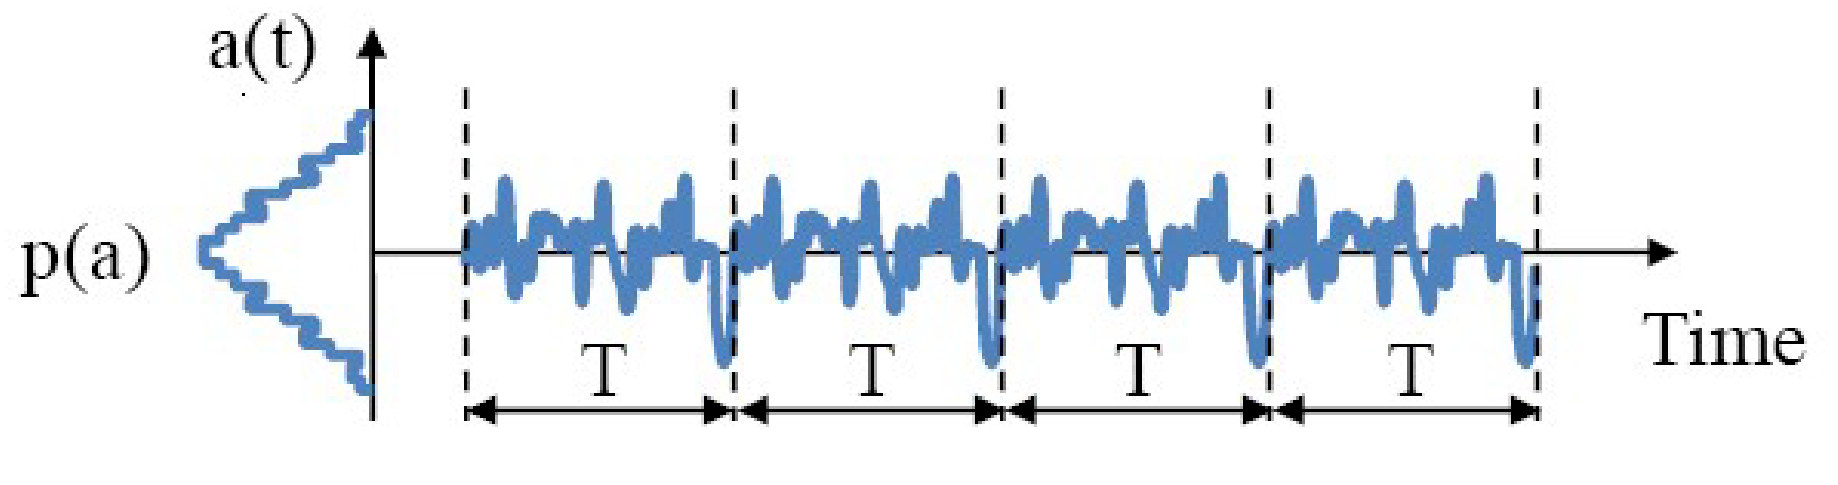
\includegraphics[width=0.6\textwidth]{p06_img01.png}
  \caption{Pseudo Random 伪随机激励信号}
  \label{fig:exp5-random}
\end{figure}

\subsection{实验测量步骤}
\begin{enumerate}
  \item 按照实验装置示意图安装试件、连接仪器、固定风力叶片，做好实验准备（已事先安装完成）。
  \item 在风力机叶片上选择贴有反光条的 15 个测点，通过钢尺量取各测点位置。
  \item 在信号发生器中选择周期 0.5 s 的 Periodic Chirp 周期线性调频脉冲激励信号。
  \item 使用仪器配套软件 InstaCal 进行数据采集，设置通道为 CH0 到 CH3，其中 CH3 为力传感器输入，CH2 为激光测振仪输出的速度通道。调节 A/D 范围为 $\pm2$ V，采样频率 5000 Hz，采样数 2048，采样模式为 Single，采样时间为 3 s。进行测试并观察各通道信号，确认采集过程顺利后，通过调节激光发射器对共 15 个测试点进行测试并记录数据。
  \item 在波形发生器中选择周期 0.5 s 的 Pseudo Random 伪随机激励信号。注意切换激励信号时要把功率放大器幅值调到最低，然后重复上一步流程。
\end{enumerate}

\section{实验测量结果}
\noindent\textbf{使用说明：}以下结果图从原报告提取，便于保留图件和读图示例。写作时请用同名文件替换为本组图像，并填写本组数据。

\subsection{测点位置}
本次实验共考虑 15 个测试点，以风机叶片底部为基准点，从下到上为正方向。测点位置如图\ref{fig:exp5-points}所示，并在表\ref{tab:exp5-points}中填写本组实际测点坐标。

\begin{figure}[H]
  \centering
  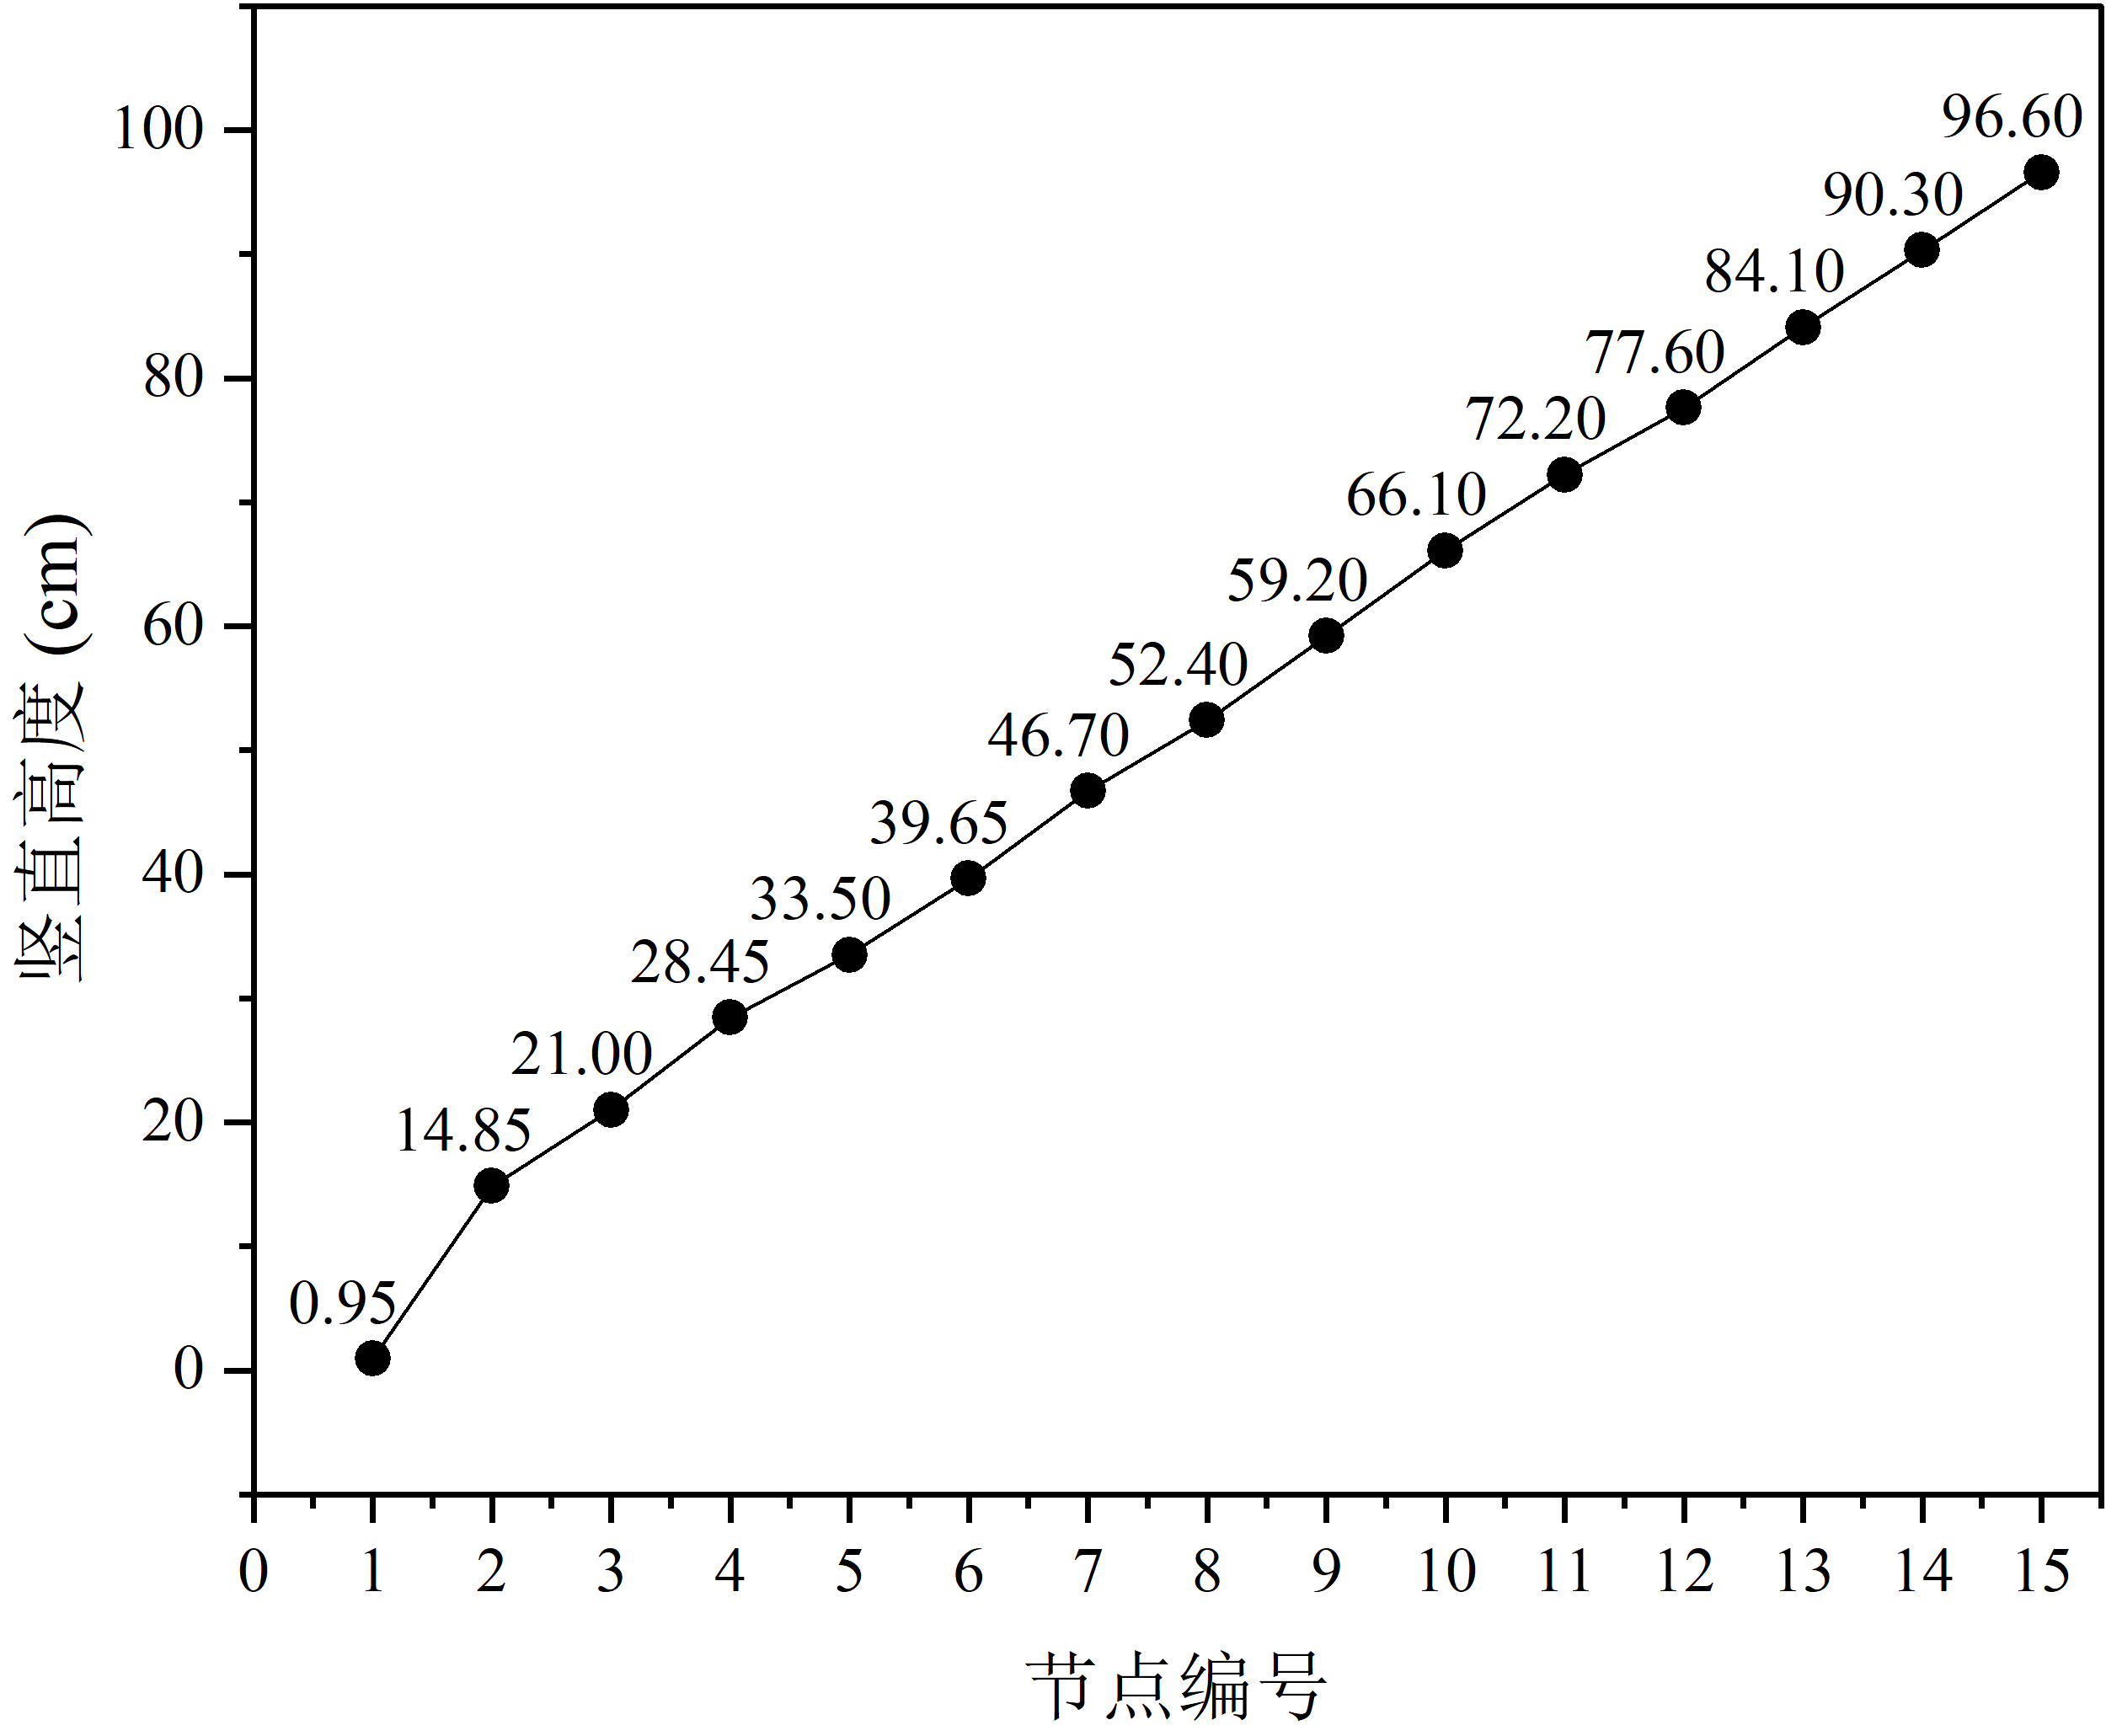
\includegraphics[width=0.52\textwidth]{p06_img02.png}
  \caption{测点位置坐标图}
  \label{fig:exp5-points}
\end{figure}

\begin{table}[H]
\centering
\caption{测点位置记录表}
\label{tab:exp5-points}
\begin{tabular}{cc|cc}
\toprule
测点 & 位置（cm） & 测点 & 位置（cm）\\
\midrule
1 & \blank[2cm] & 9 & \blank[2cm]\\
2 & \blank[2cm] & 10 & \blank[2cm]\\
3 & \blank[2cm] & 11 & \blank[2cm]\\
4 & \blank[2cm] & 12 & \blank[2cm]\\
5 & \blank[2cm] & 13 & \blank[2cm]\\
6 & \blank[2cm] & 14 & \blank[2cm]\\
7 & \blank[2cm] & 15 & \blank[2cm]\\
8 & \blank[2cm] & \multicolumn{2}{c}{——}\\
\bottomrule
\end{tabular}
\end{table}

\subsection{Periodic Chirp 信号处理}
首先分析周期线性调频脉冲激励信号（Periodic Chirp）。为确保实验结果准确，每个测点进行三次重复测量。通过对输入和输出信号进行快速傅里叶变换（FFT），并将输出信号与输入信号进行除法处理，得到每个测点的平均频响函数。在信号处理过程中采用矩形窗函数，以减少频谱泄漏效应。

由于输出信号为风机叶片上各测点的速度信号，通过分析频响函数的实频域部分确定固有频率、模态和阻尼比。实频曲线如图\ref{fig:exp5-chirp-real}所示。

\begin{figure}[H]
  \centering
  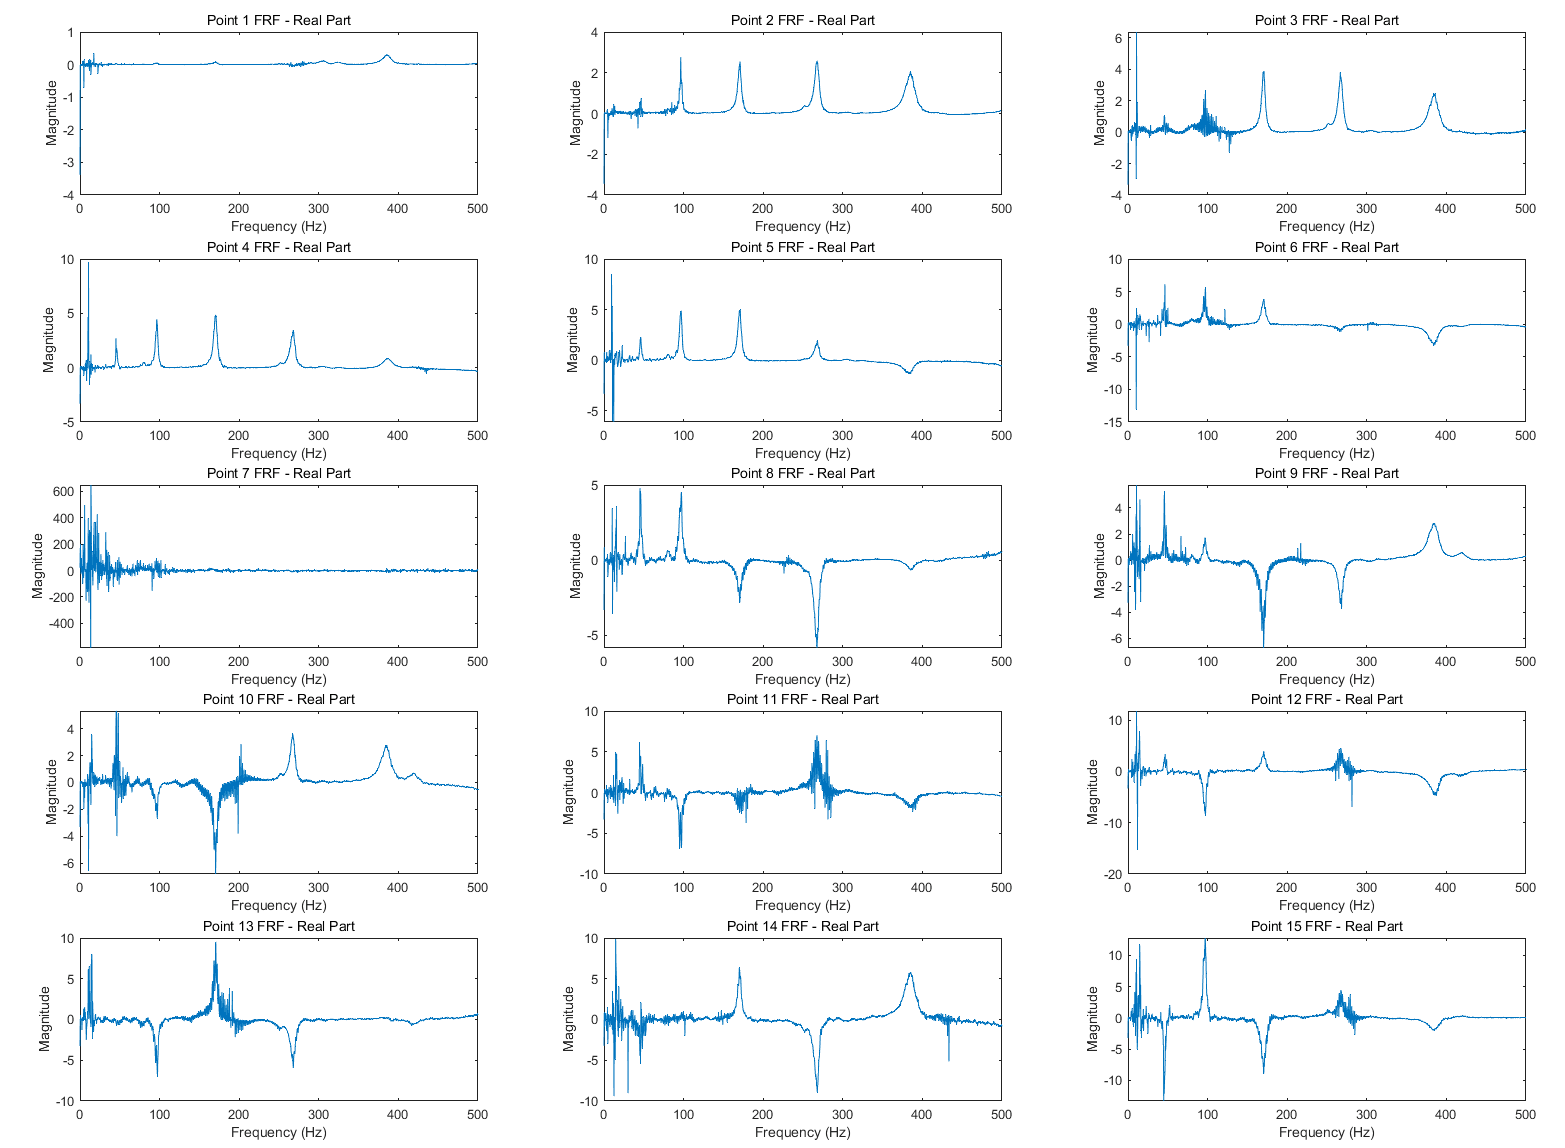
\includegraphics[width=0.9\textwidth]{p07_img01.png}
  \caption{Periodic Chirp 输入信号对应的平均实域曲线}
  \label{fig:exp5-chirp-real}
\end{figure}

根据实频域曲线峰值对应的频率确定固有频率，并通过半功率点法计算前五阶固有频率和阻尼比，填入表\ref{tab:exp5-chirp-results}。

\begin{table}[H]
\centering\small
\caption{Periodic Chirp 输入信号对应的固有频率与阻尼率}
\label{tab:exp5-chirp-results}
\begin{tabular}{lccccc}
\toprule
阶数 & 一阶 & 二阶 & 三阶 & 四阶 & 五阶\\
\midrule
固有频率（Hz） & \blank[1.2cm] & \blank[1.2cm] & \blank[1.2cm] & \blank[1.2cm] & \blank[1.2cm]\\
阻尼率 & \blank[1.2cm] & \blank[1.2cm] & \blank[1.2cm] & \blank[1.2cm] & \blank[1.2cm]\\
\bottomrule
\end{tabular}
\end{table}

将各阶固有频率下各测点处的实频峰值相连，得到风机叶片振动时的各阶振型。将最下面的节点位移归一化为 1，并对其他节点位移进行等比例缩放，得到前五阶模态的归一化振型图，如图\ref{fig:exp5-chirp-modes}所示。

\begin{figure}[H]
\centering
\subcaptionbox{一阶模态}[0.42\textwidth]{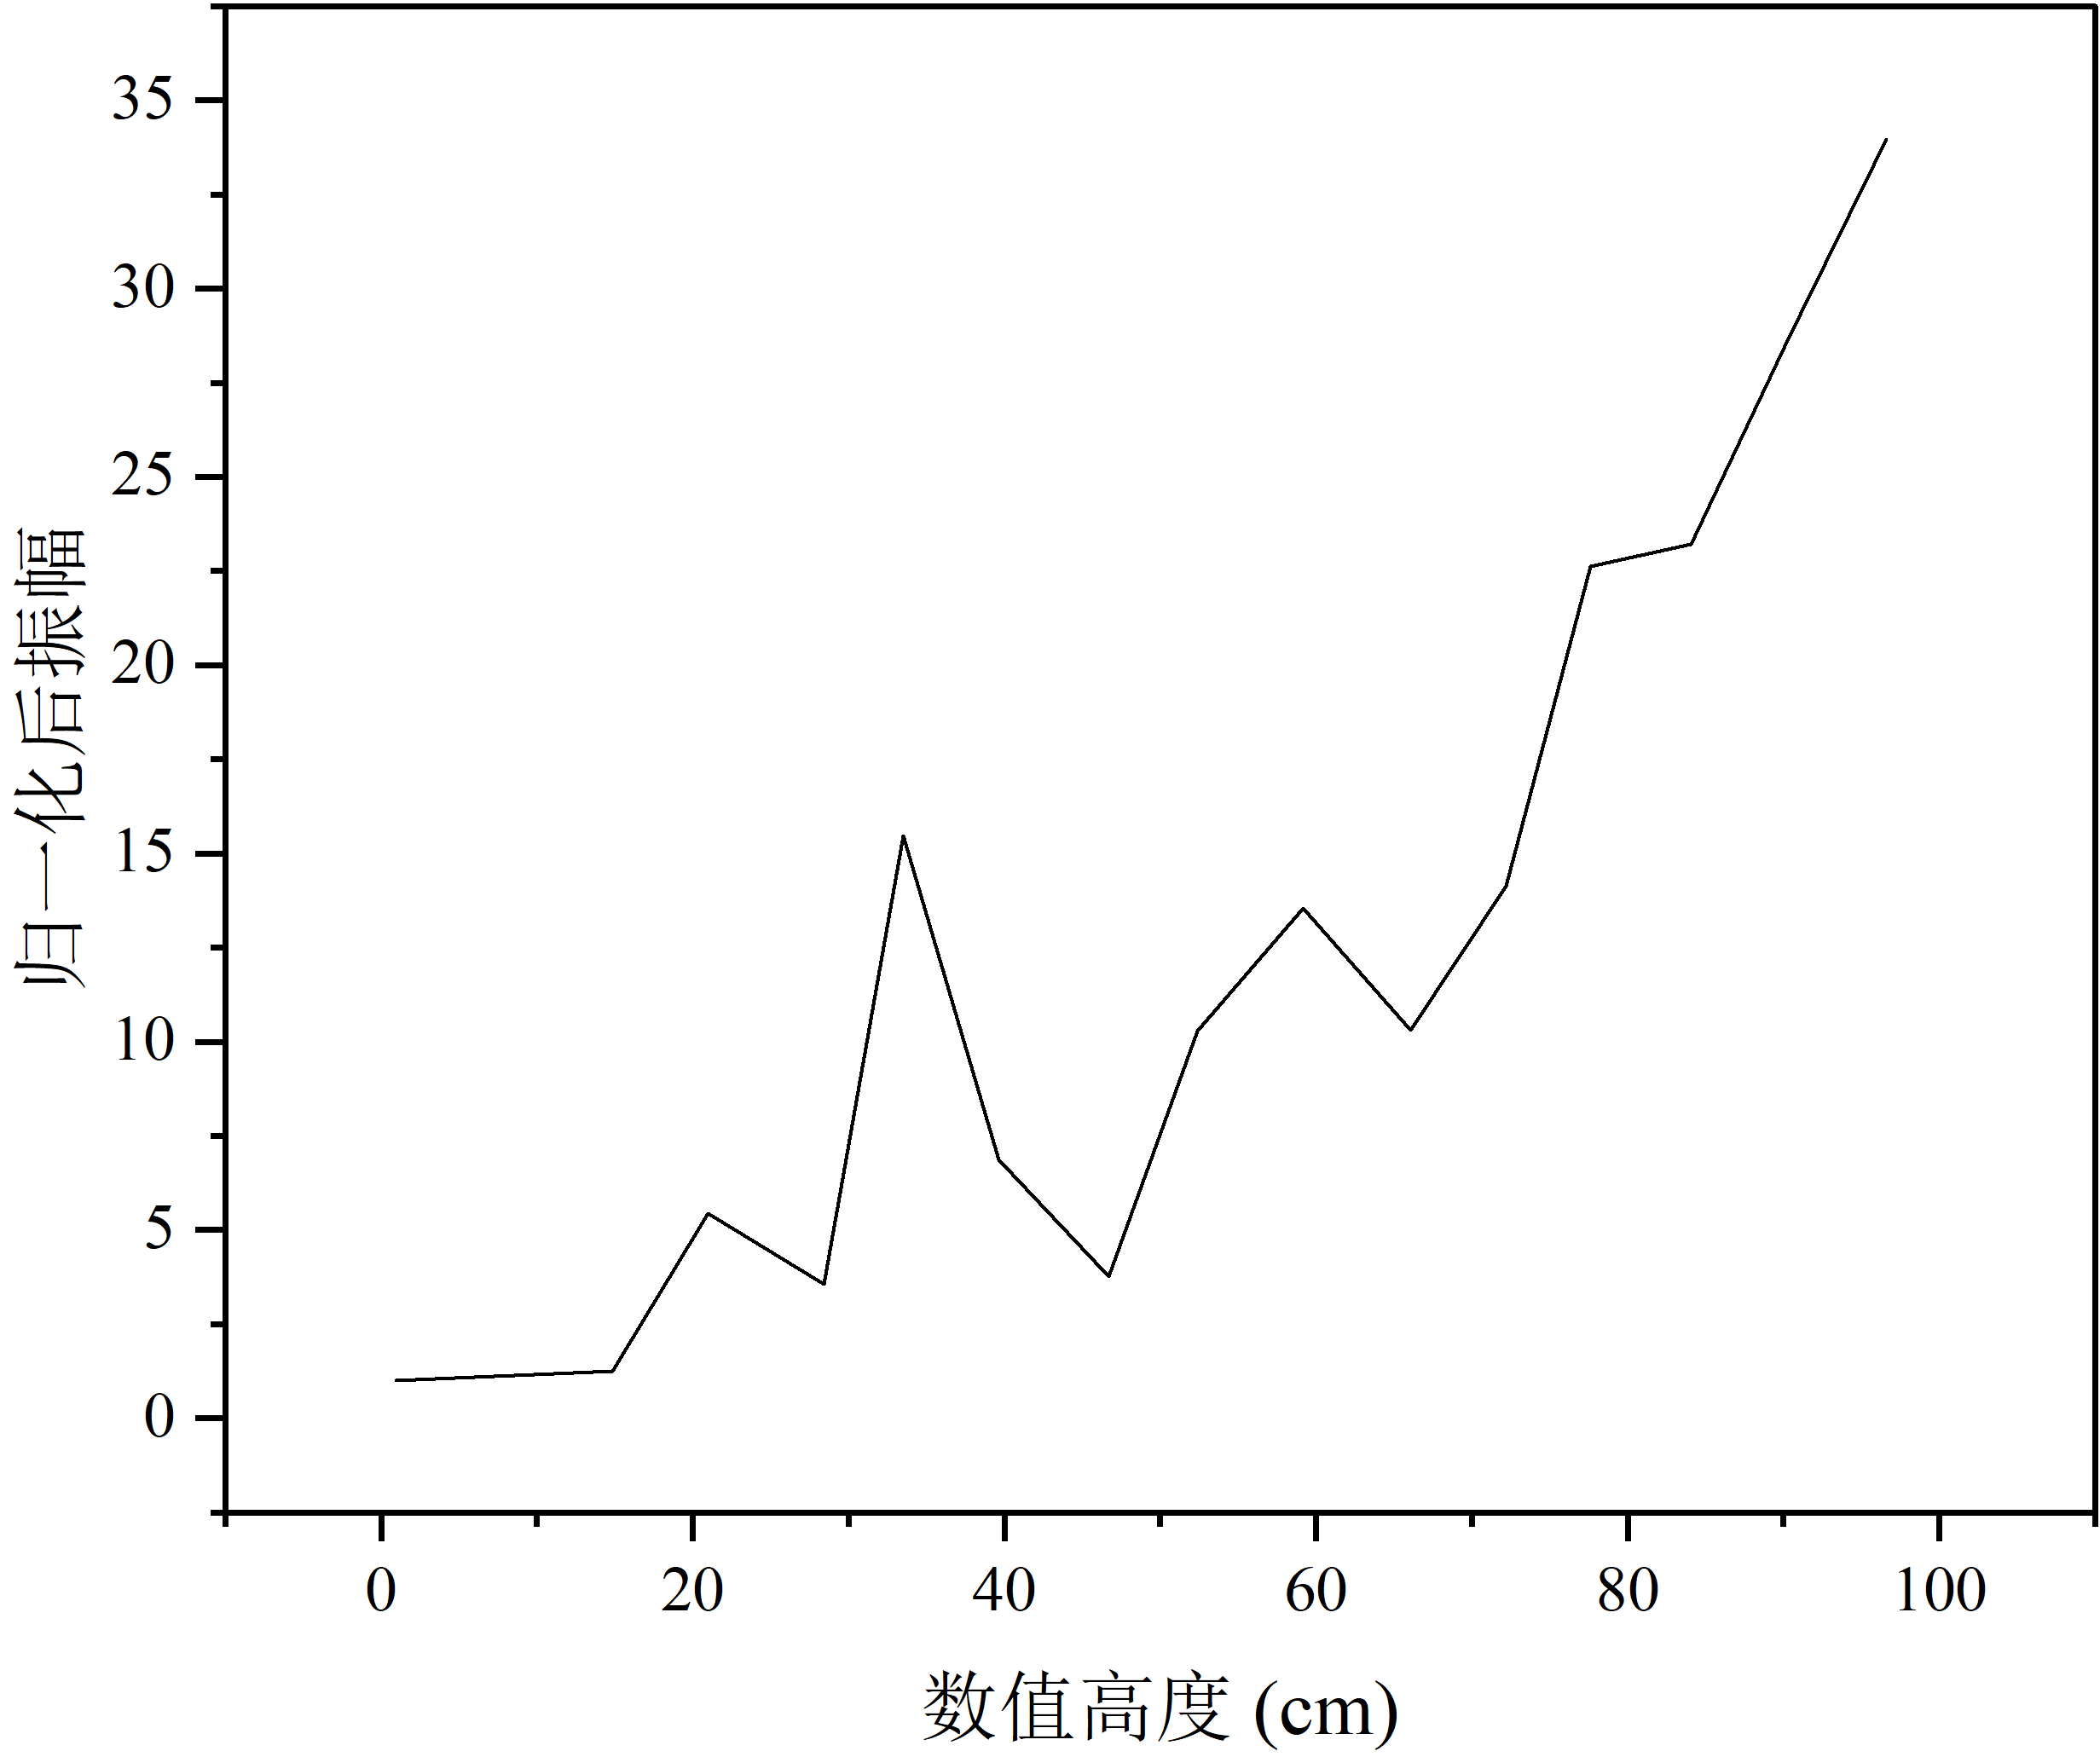
\includegraphics[width=\linewidth]{p08_img01.png}}\hfill
\subcaptionbox{二阶模态}[0.42\textwidth]{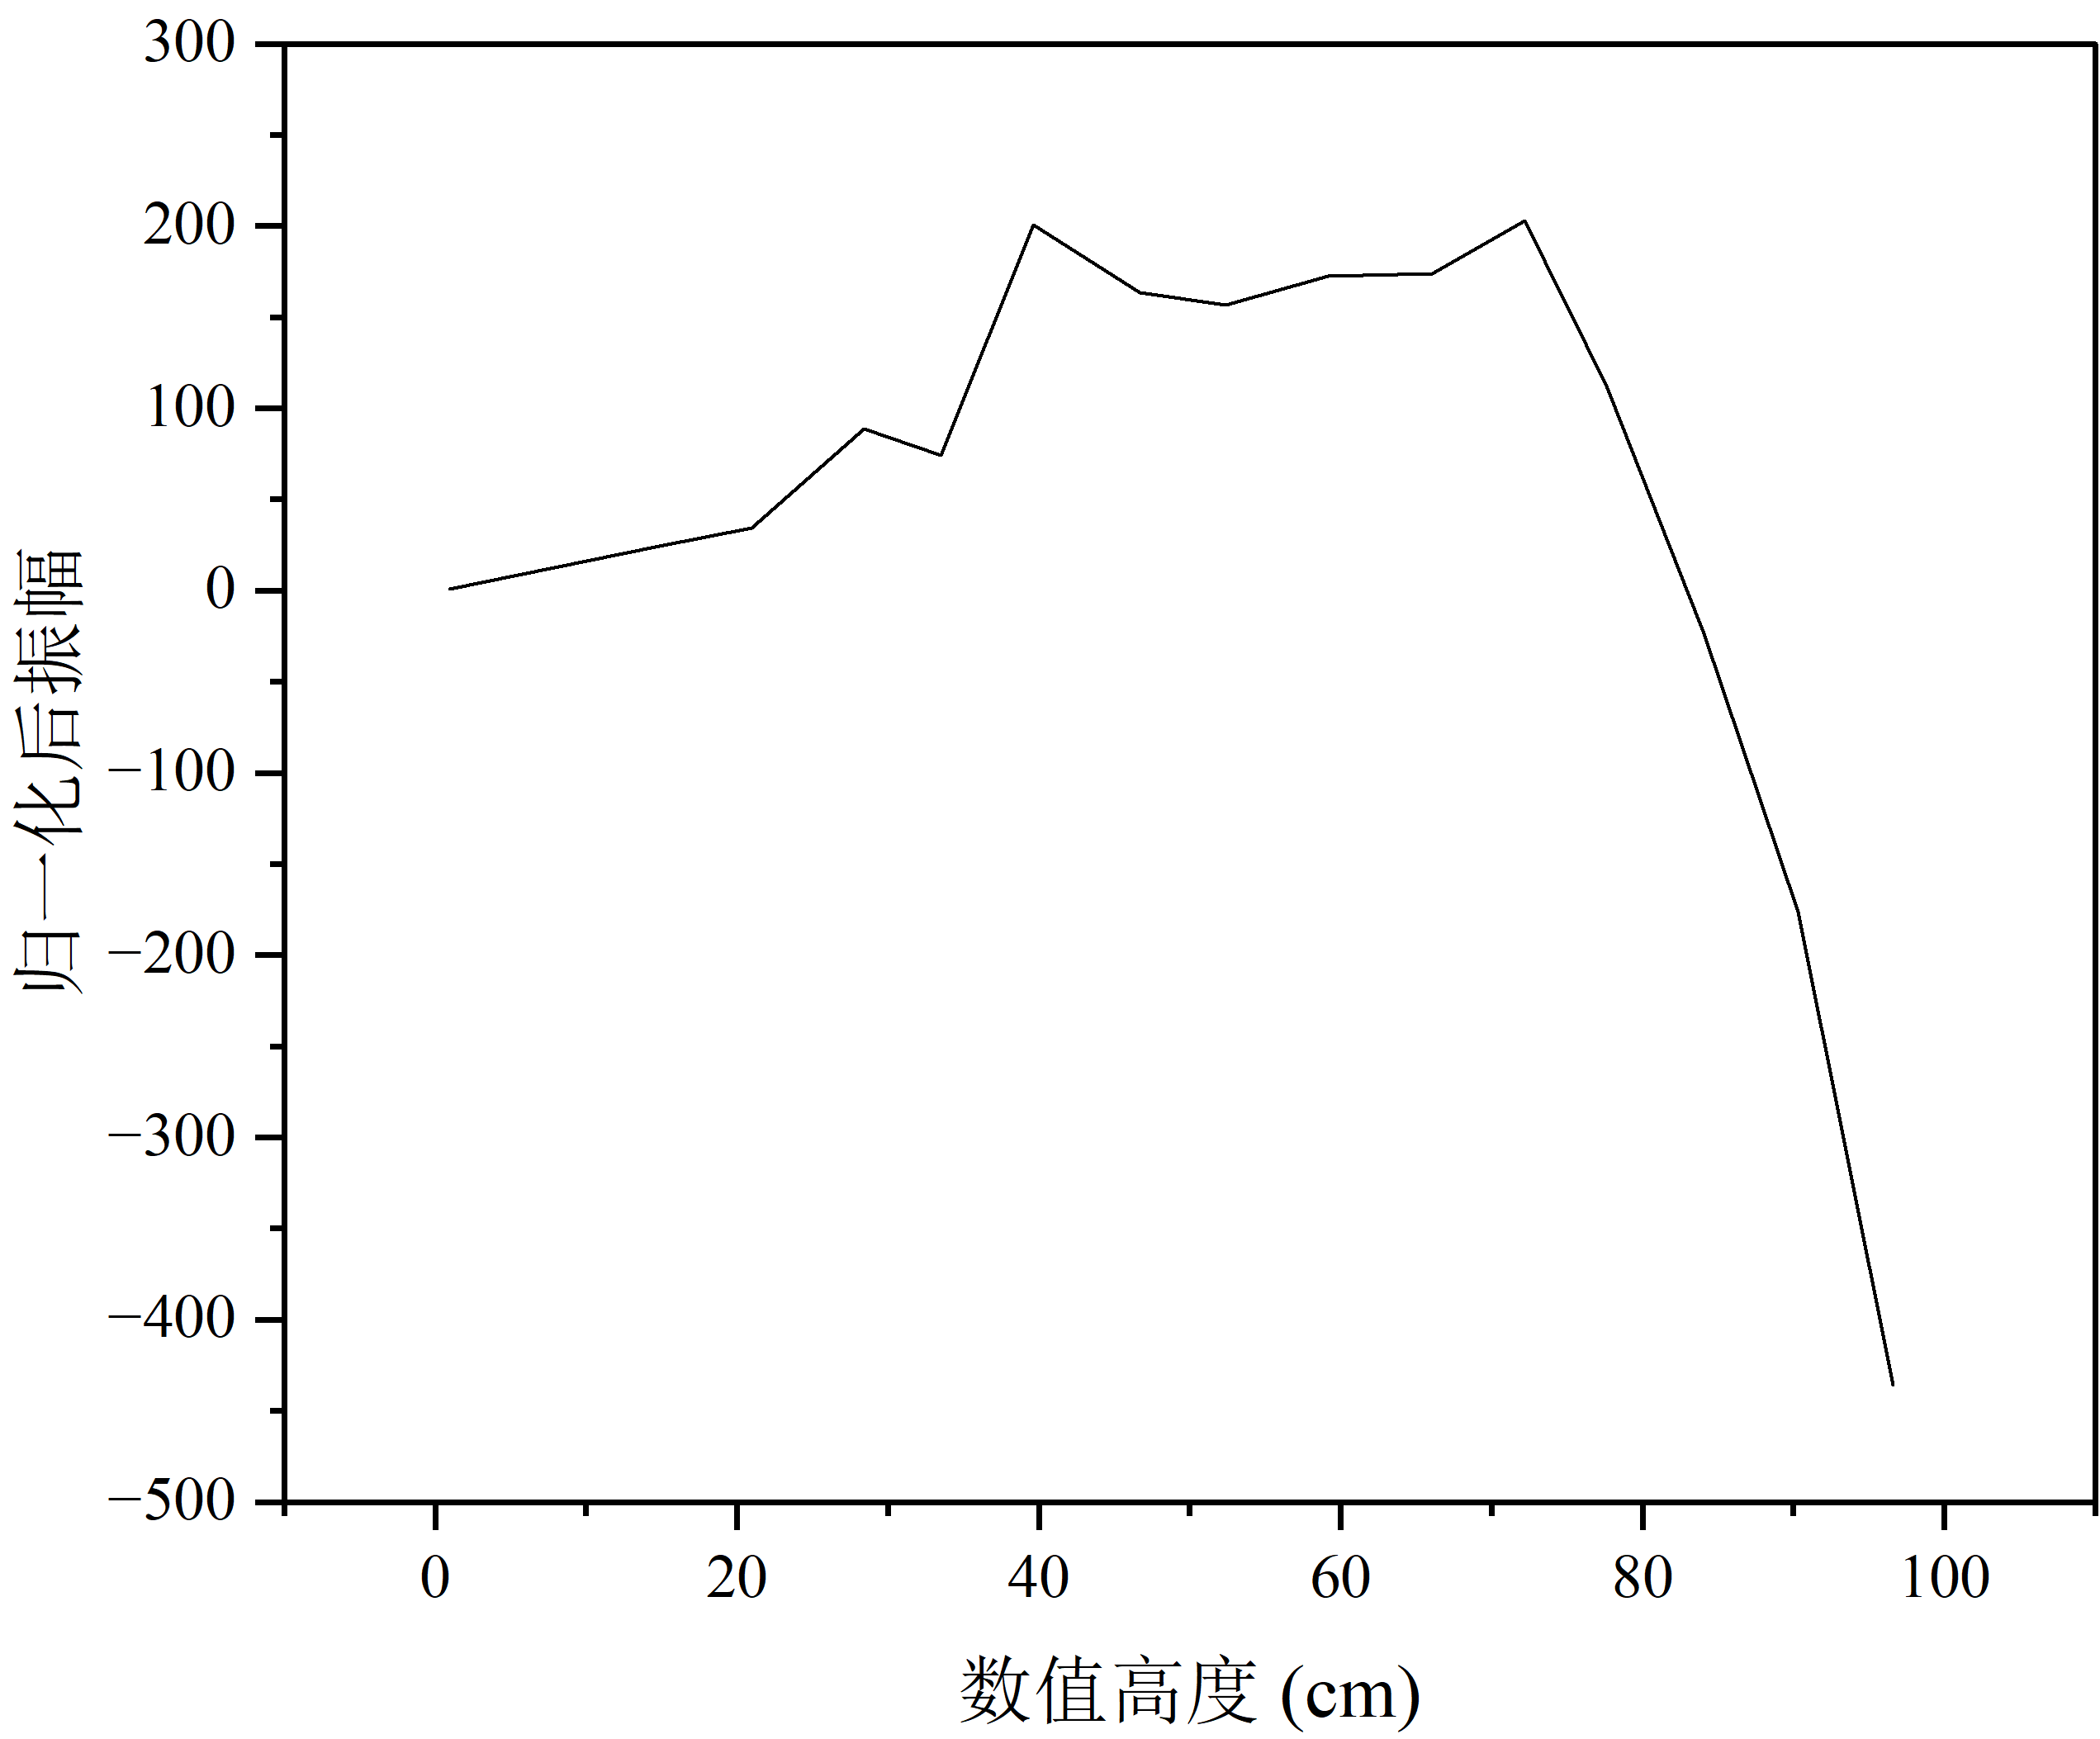
\includegraphics[width=\linewidth]{p08_img02.png}}\\[0.5em]
\subcaptionbox{三阶模态}[0.42\textwidth]{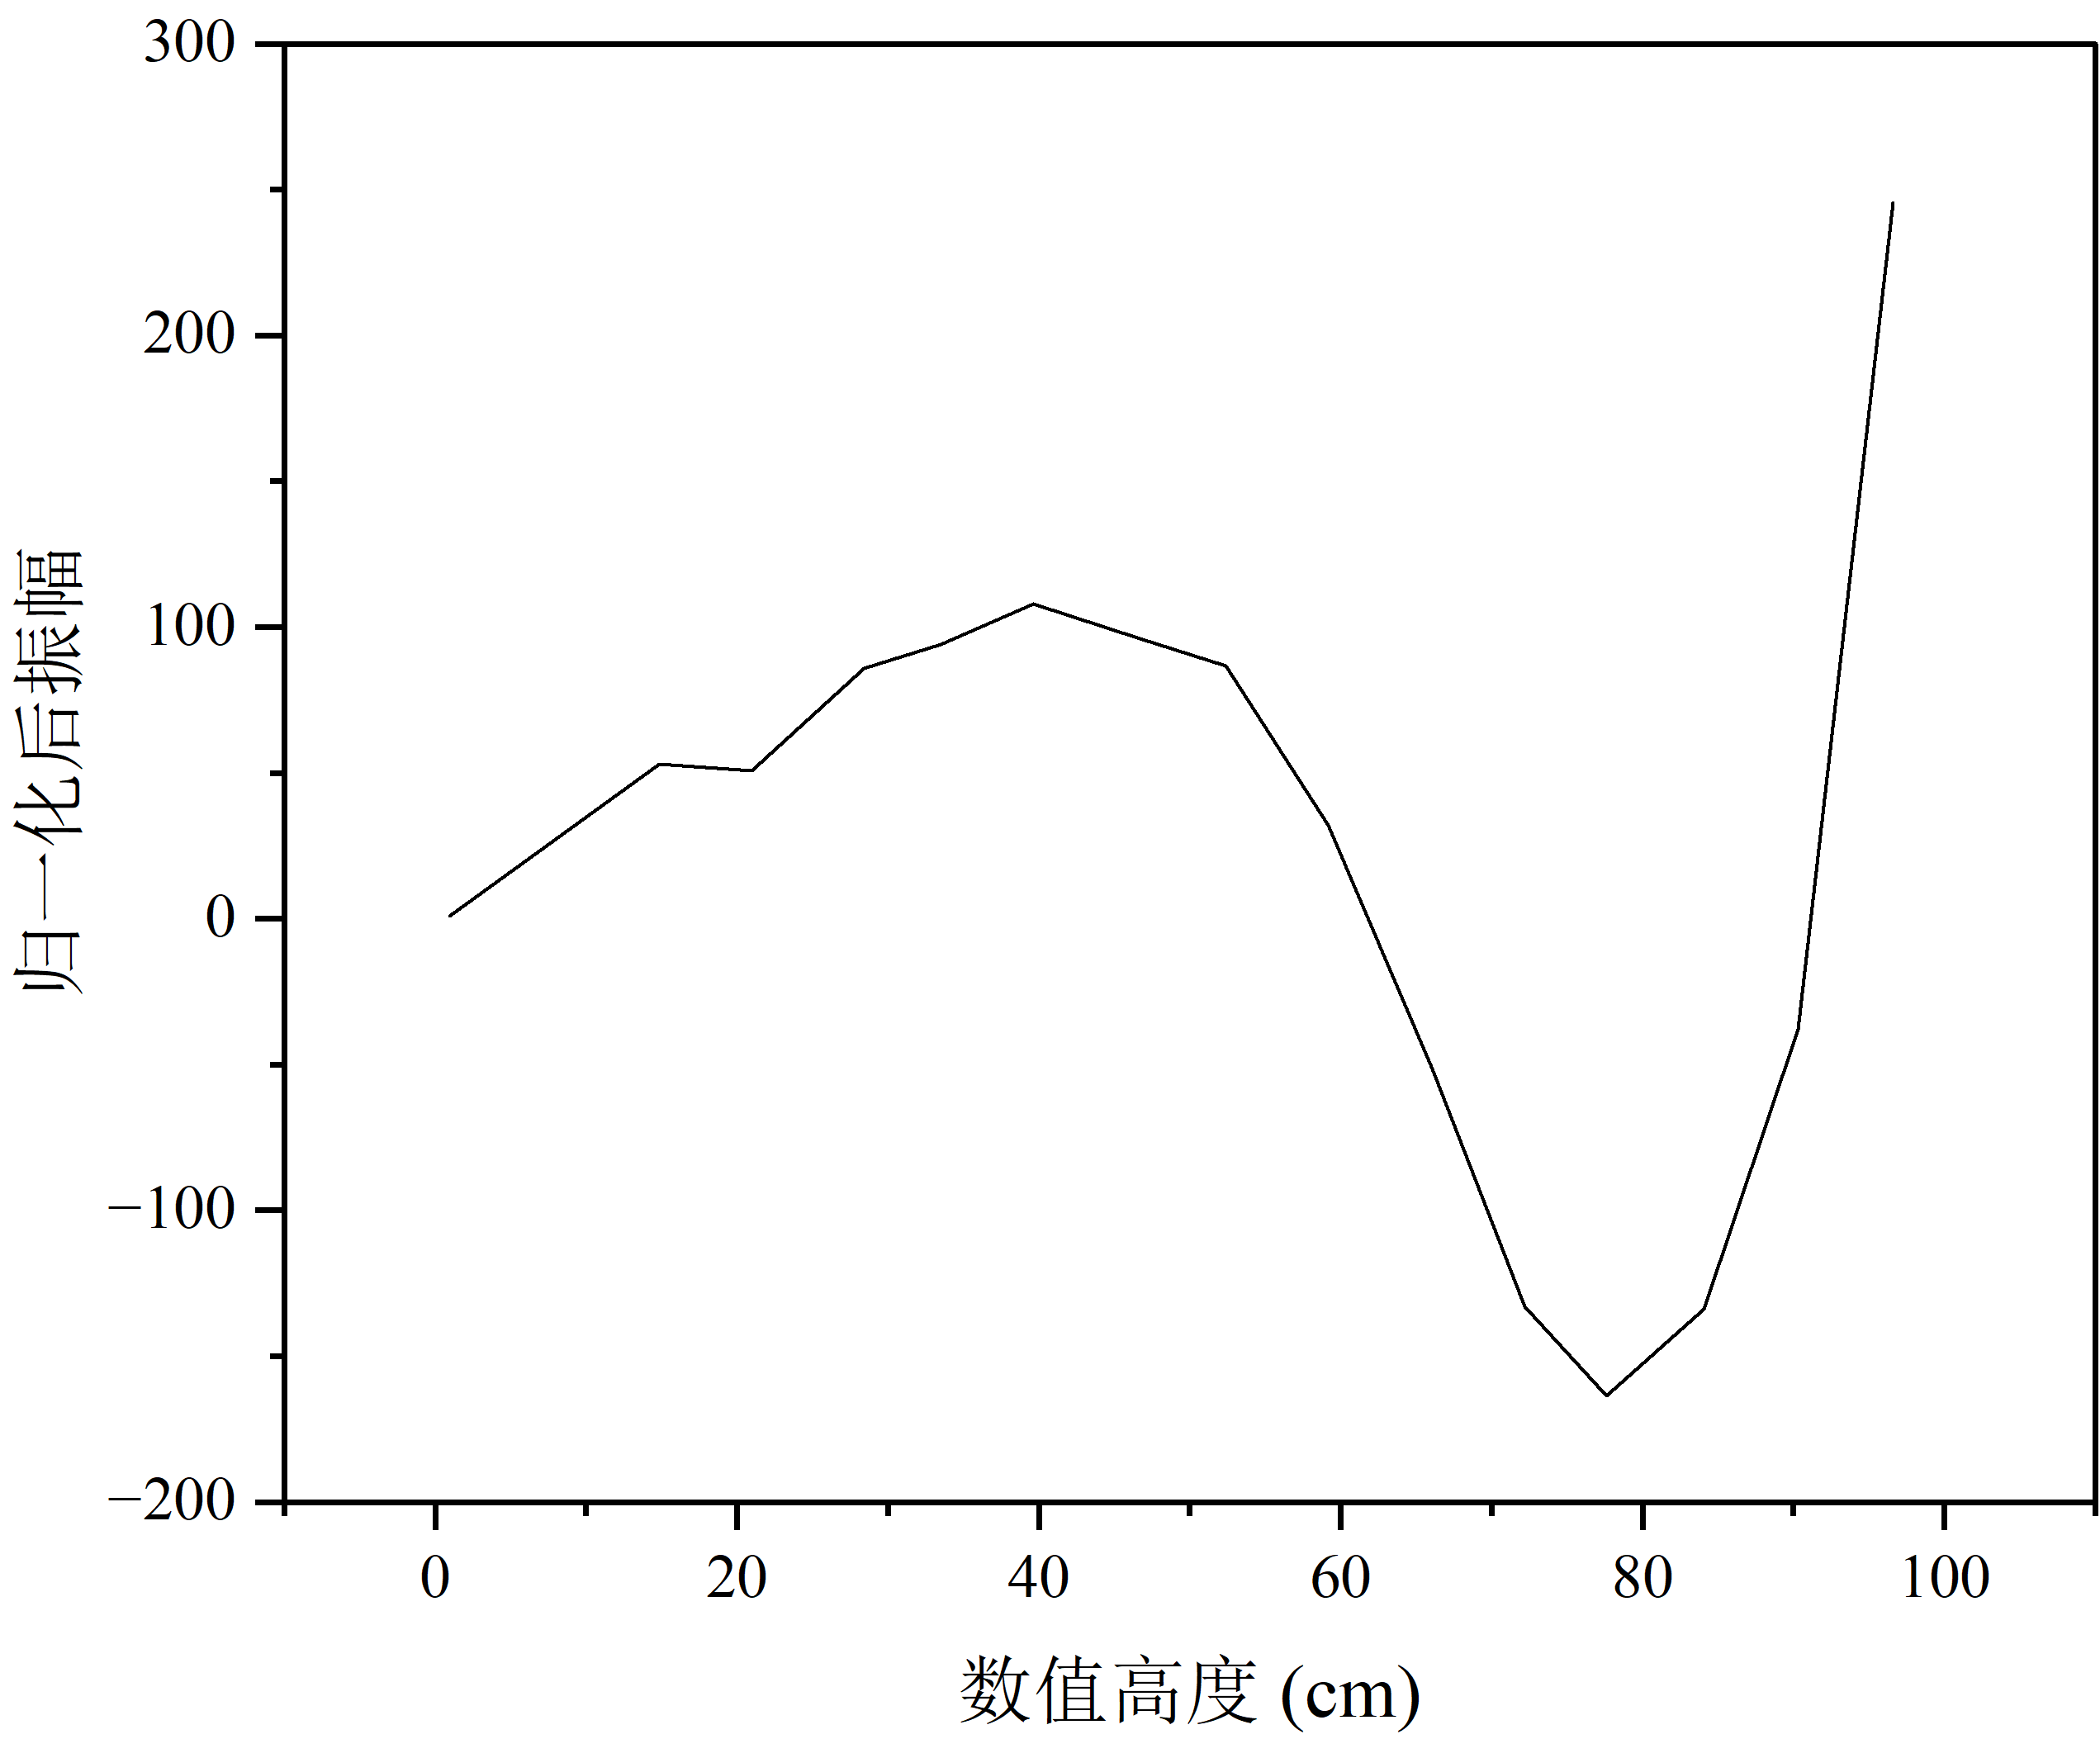
\includegraphics[width=\linewidth]{p08_img03.png}}\hfill
\subcaptionbox{四阶模态}[0.42\textwidth]{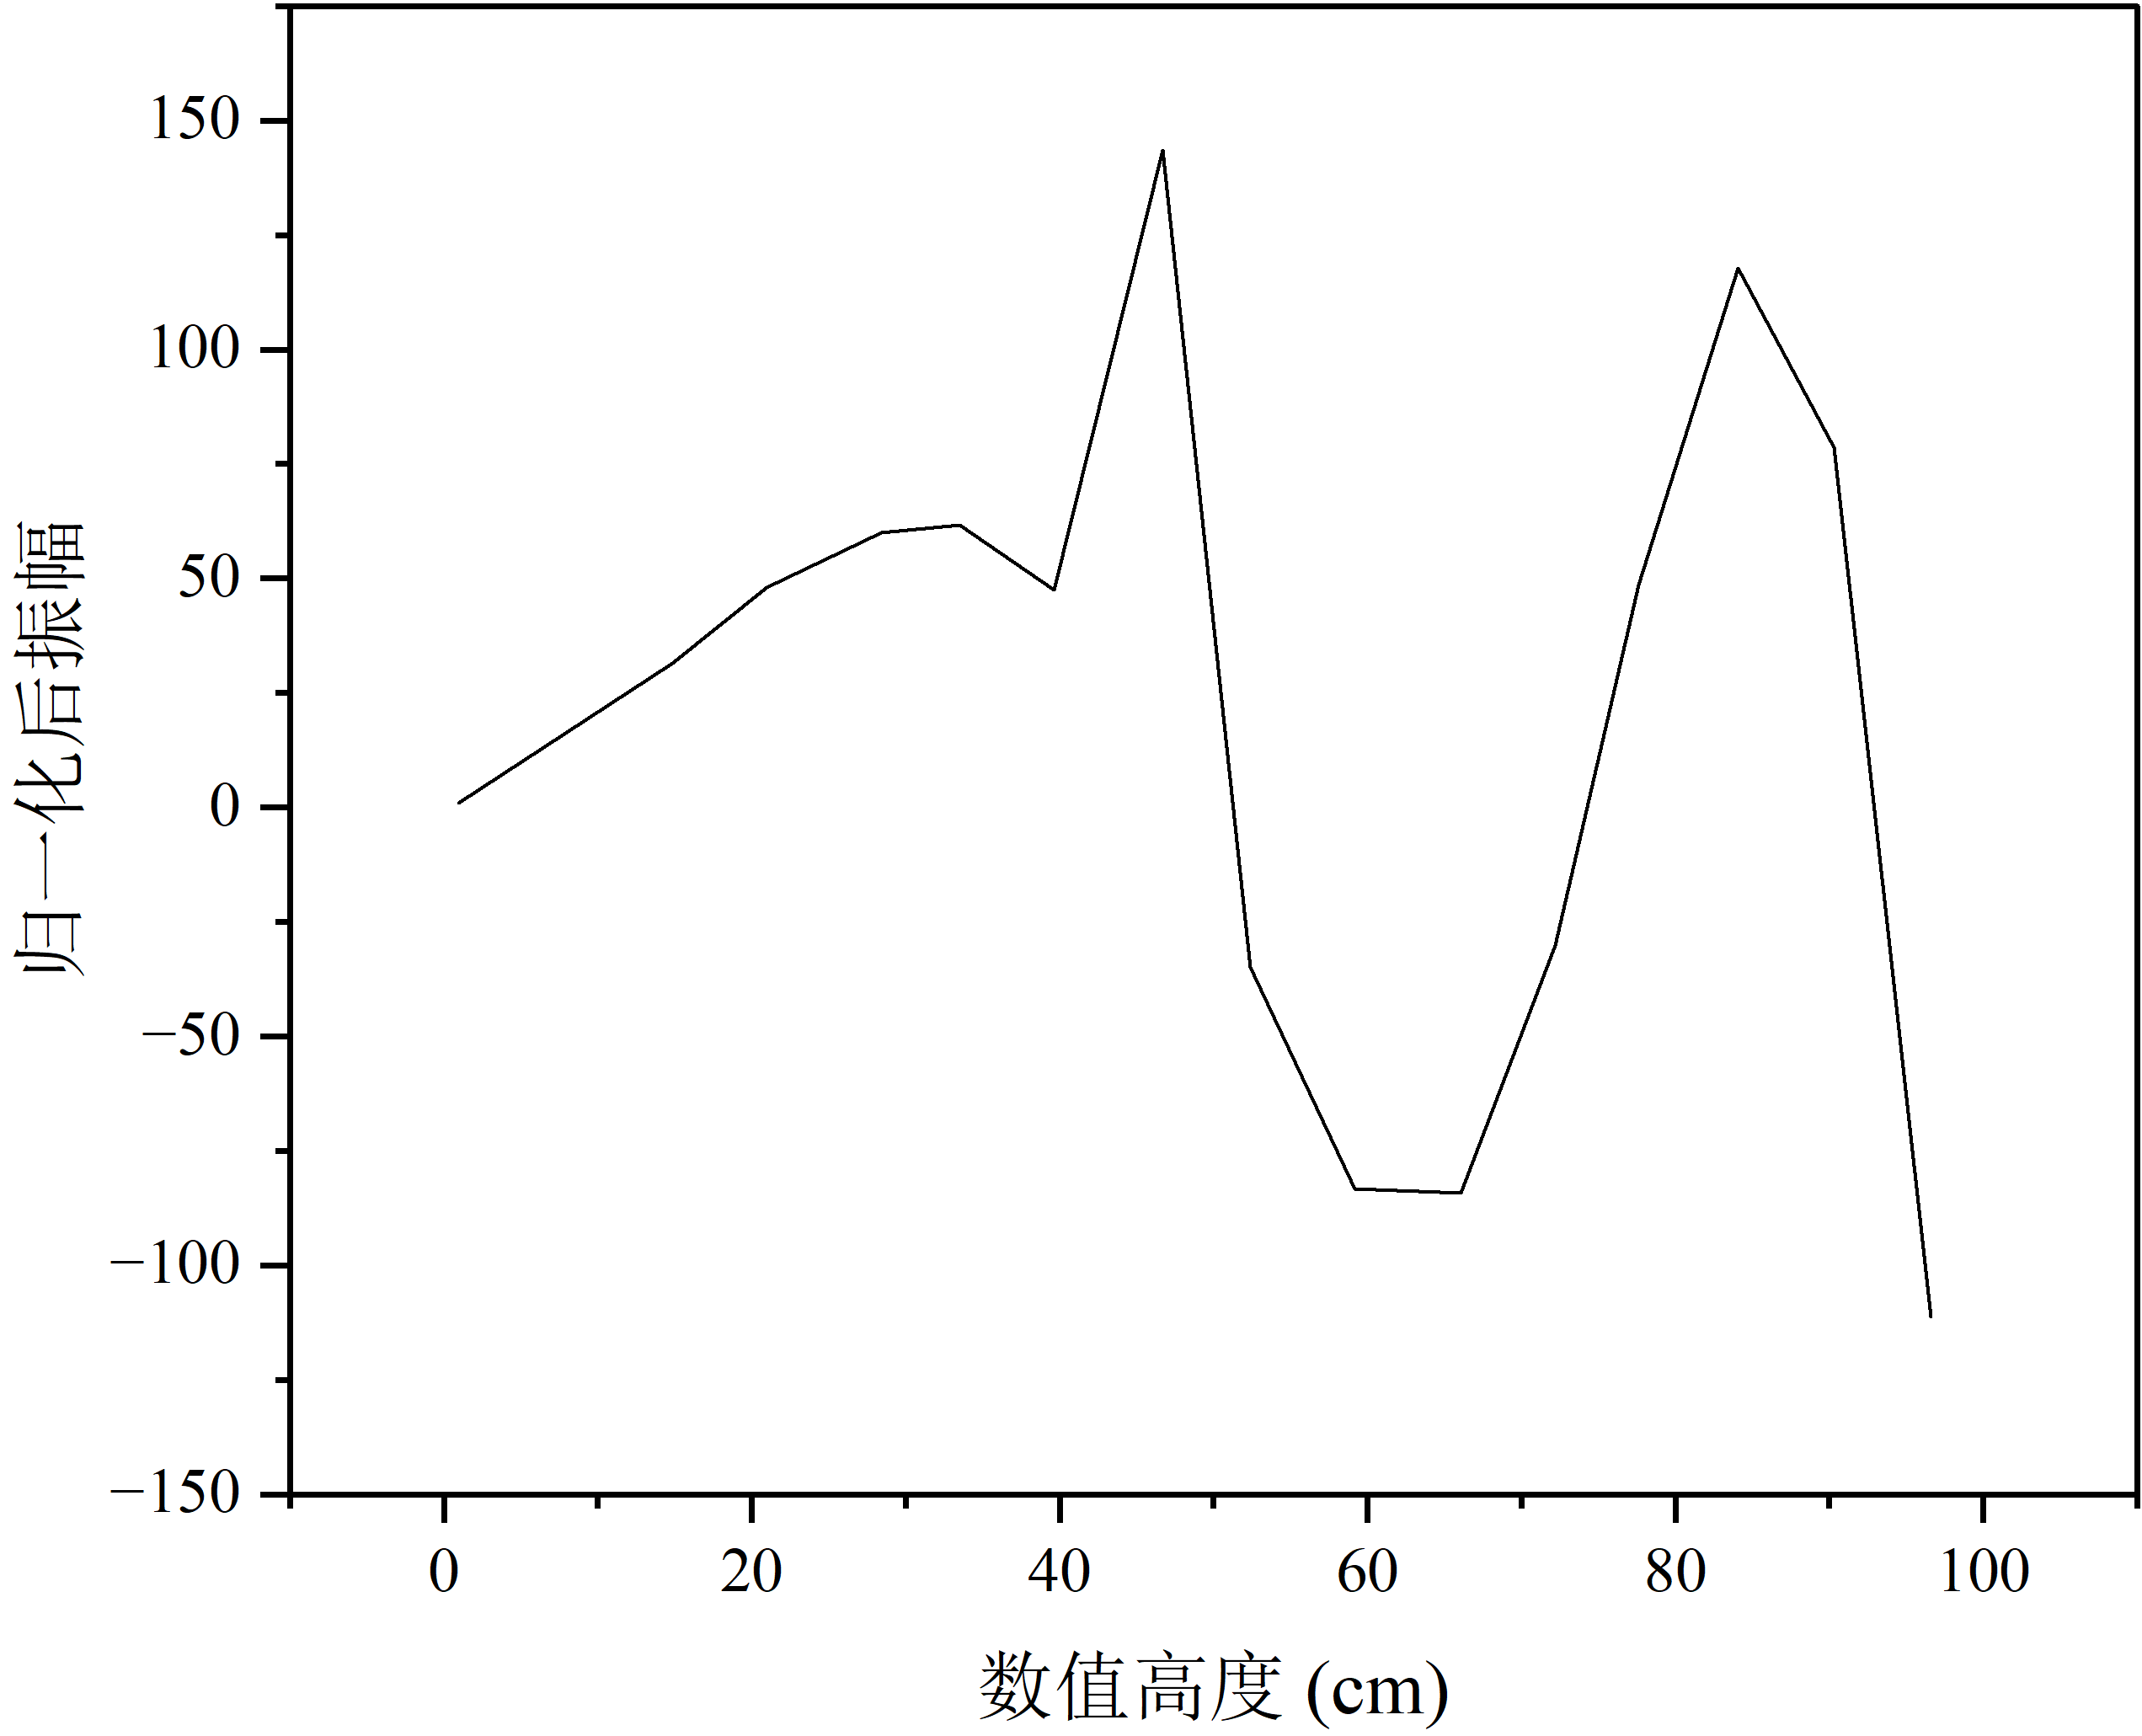
\includegraphics[width=\linewidth]{p08_img04.png}}\\[0.5em]
\subcaptionbox{五阶模态}[0.42\textwidth]{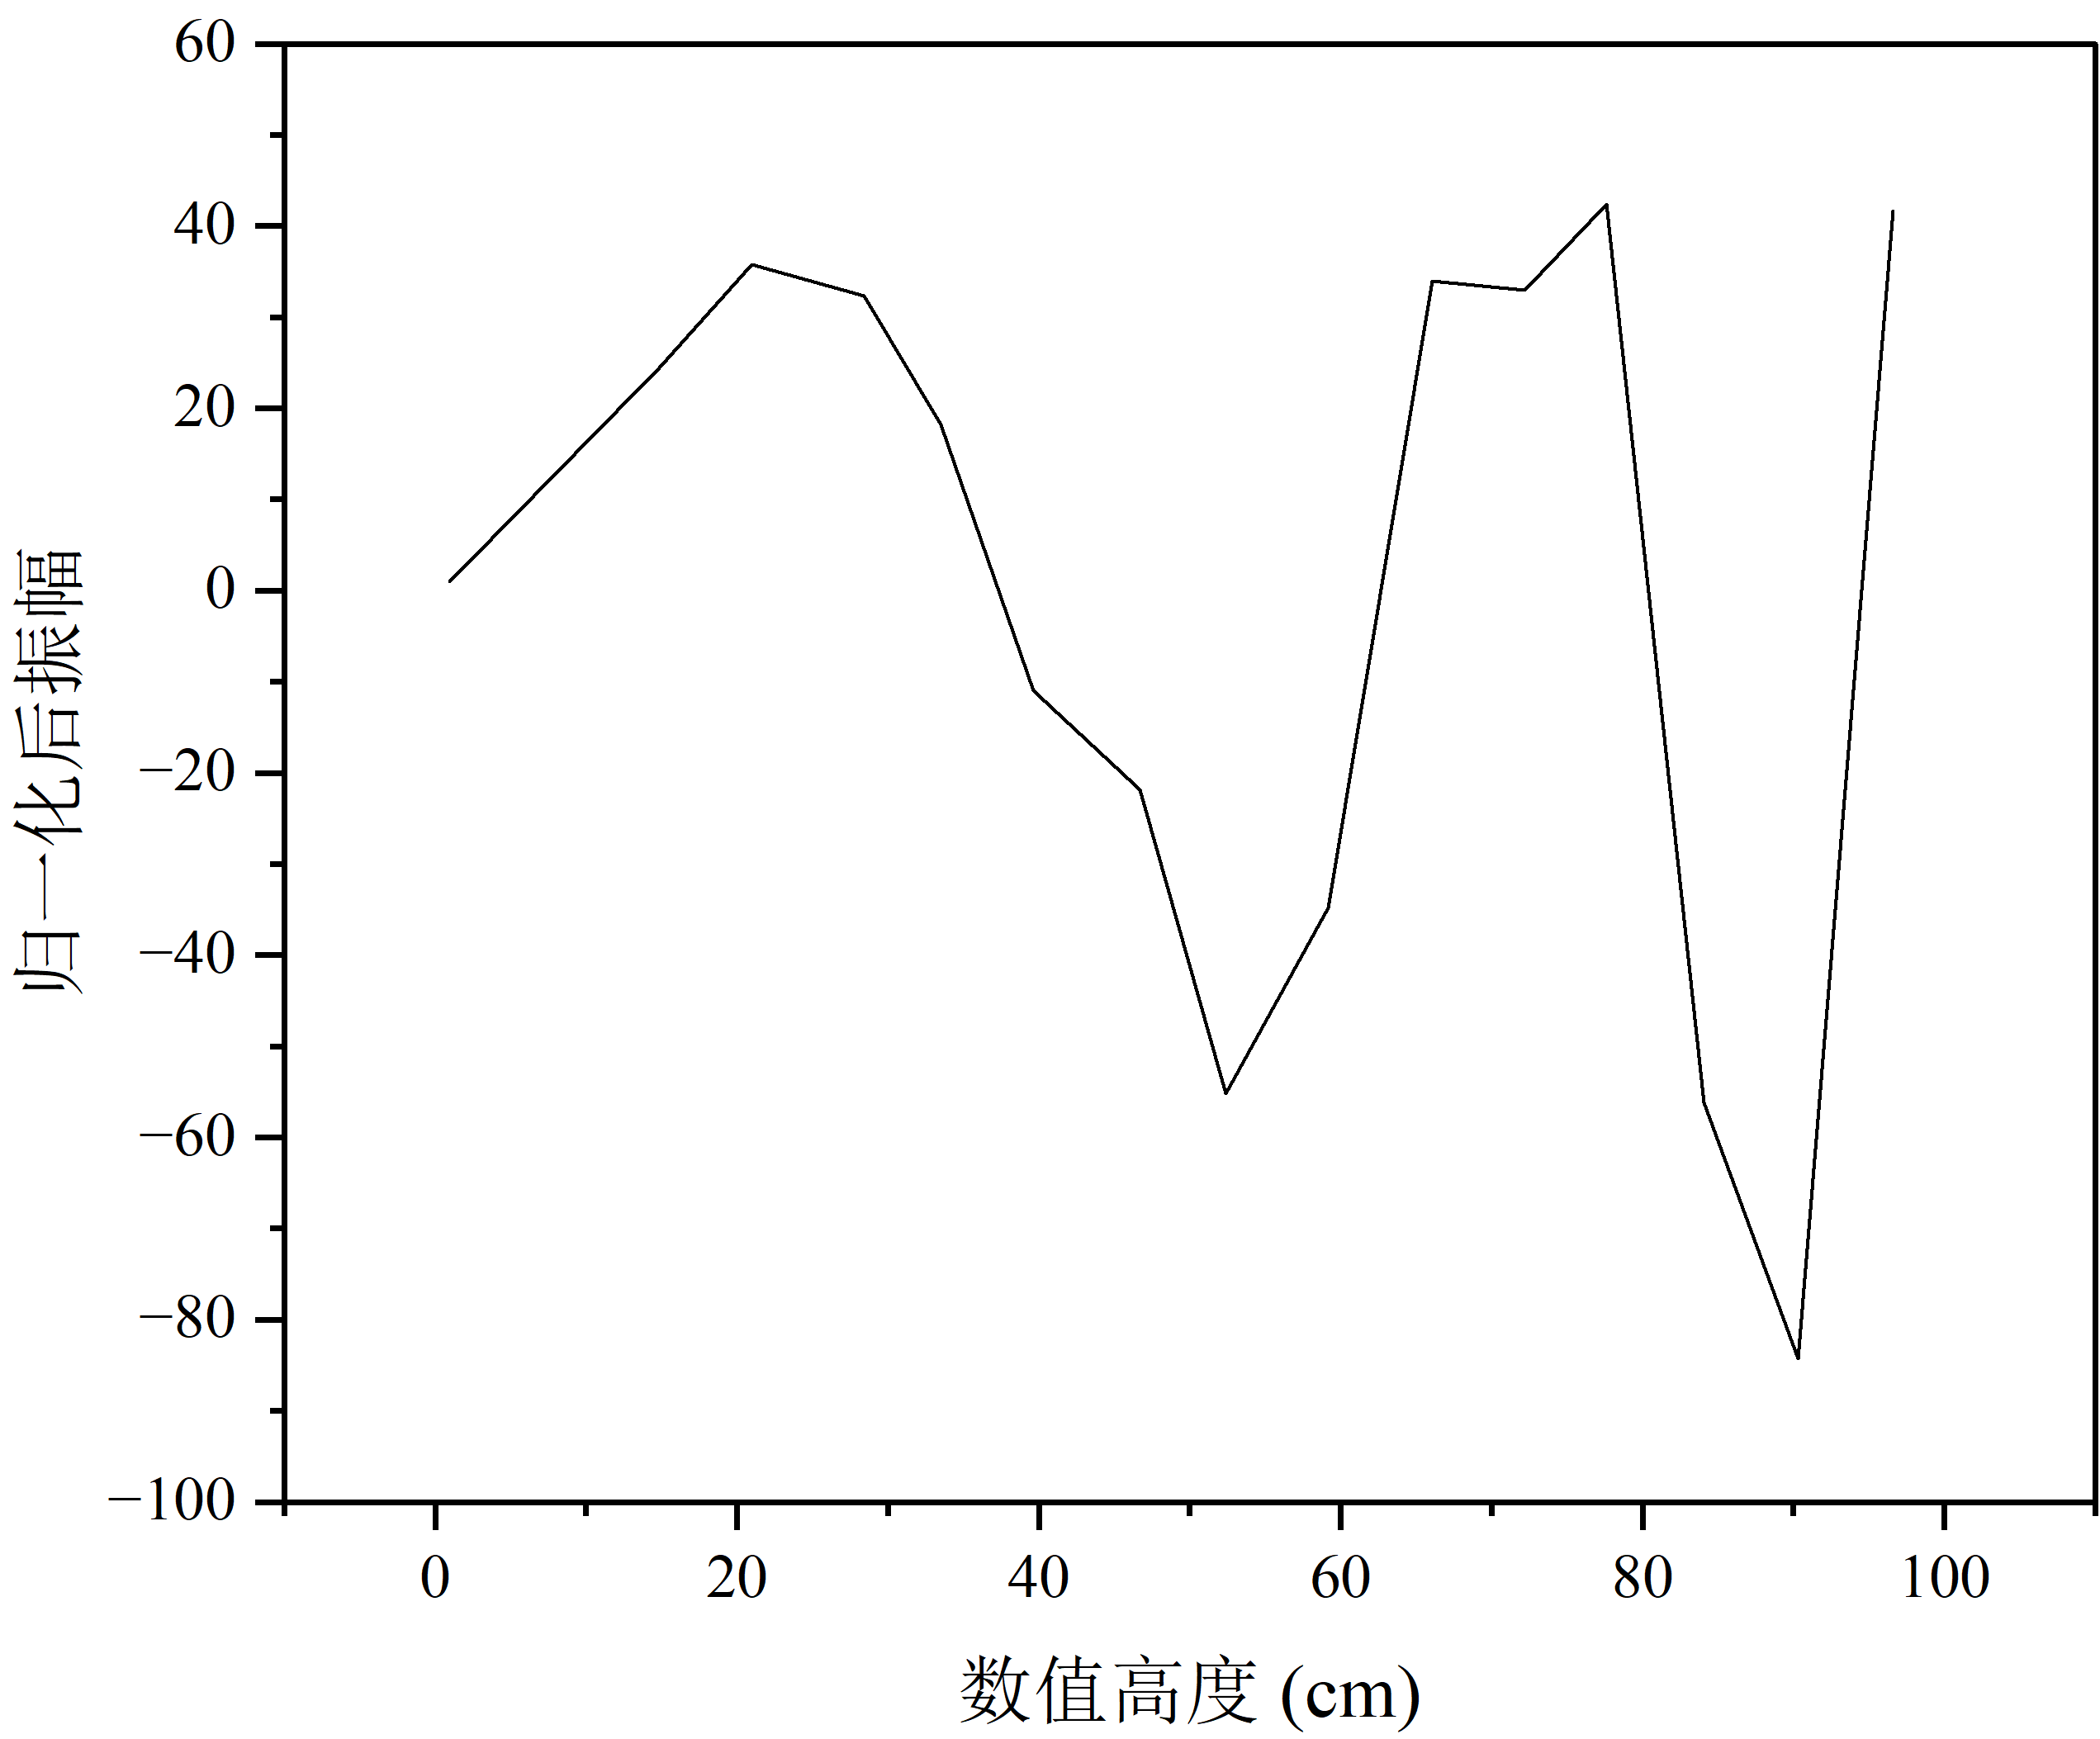
\includegraphics[width=\linewidth]{p08_img05.png}}
\caption{Periodic Chirp 输入信号对应的前五阶固有模态}
\label{fig:exp5-chirp-modes}
\end{figure}

\subsection{Pseudo Random 信号处理}
接下来分析伪随机激励信号（Pseudo Random）。与周期线性调频脉冲激励信号一样，每个测点进行三次重复测量。通过对输入和输出信号进行 FFT，并将输出信号与输入信号进行除法处理，得到每个测点的平均频响函数。在信号处理过程中采用矩形窗以减少频谱泄漏。

由于输出信号为风机叶片上各测点的速度信号，通过分析频响函数的实频域部分确定固有频率、模态和阻尼比。实频曲线如图\ref{fig:exp5-random-real}所示。

\begin{figure}[H]
  \centering
  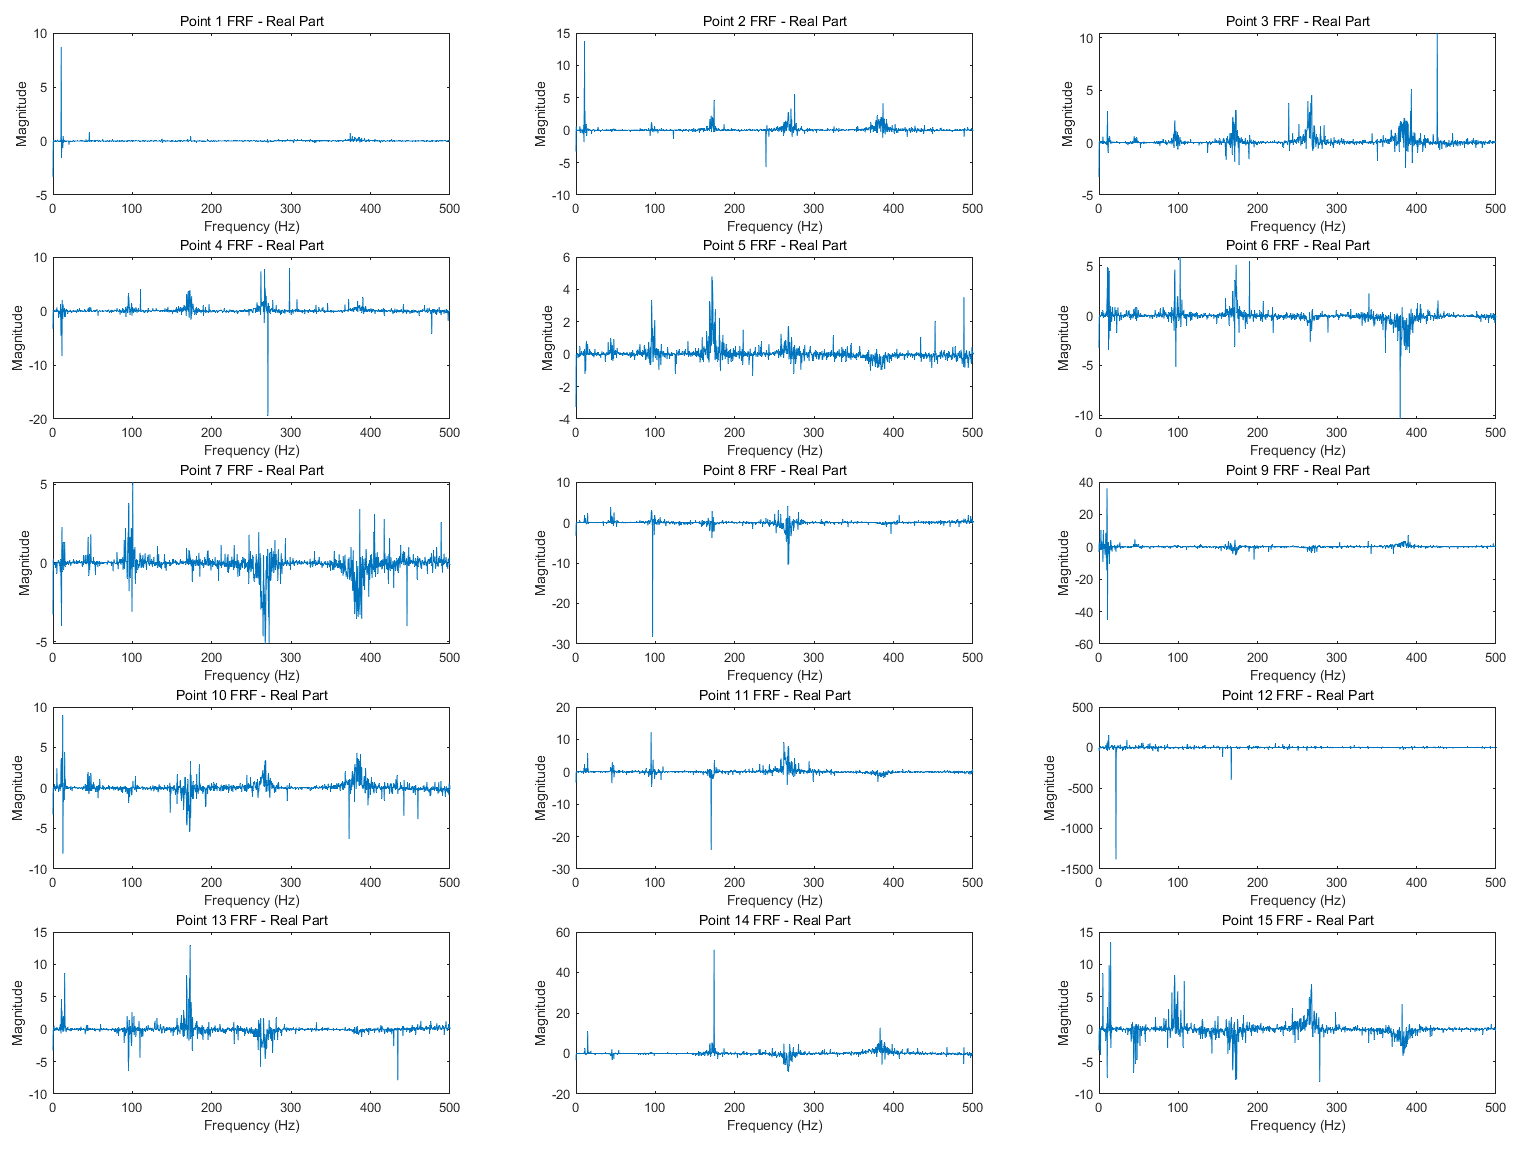
\includegraphics[width=0.9\textwidth]{p09_img01.png}
  \caption{Pseudo Random 输入信号对应的平均实域曲线}
  \label{fig:exp5-random-real}
\end{figure}

与前述相同，通过分析实频域曲线峰值对应的频率得到前五阶固有频率和阻尼比，填入表\ref{tab:exp5-random-results}。

\begin{table}[H]
\centering\small
\caption{Pseudo Random 输入信号对应的固有频率与阻尼率}
\label{tab:exp5-random-results}
\begin{tabular}{lccccc}
\toprule
阶数 & 一阶 & 二阶 & 三阶 & 四阶 & 五阶\\
\midrule
固有频率（Hz） & \blank[1.2cm] & \blank[1.2cm] & \blank[1.2cm] & \blank[1.2cm] & \blank[1.2cm]\\
阻尼率 & \blank[1.2cm] & \blank[1.2cm] & \blank[1.2cm] & \blank[1.2cm] & \blank[1.2cm]\\
\bottomrule
\end{tabular}
\end{table}

将各阶固有频率下各测点处的实频峰值相连，得到风机叶片振动时的各阶振型。将最下面的节点位移归一化为 1，并对其他节点位移进行等比例缩放，得到前五阶模态的归一化振型图，如图\ref{fig:exp5-random-modes}所示。

\begin{figure}[H]
\centering
\subcaptionbox{一阶模态}[0.42\textwidth]{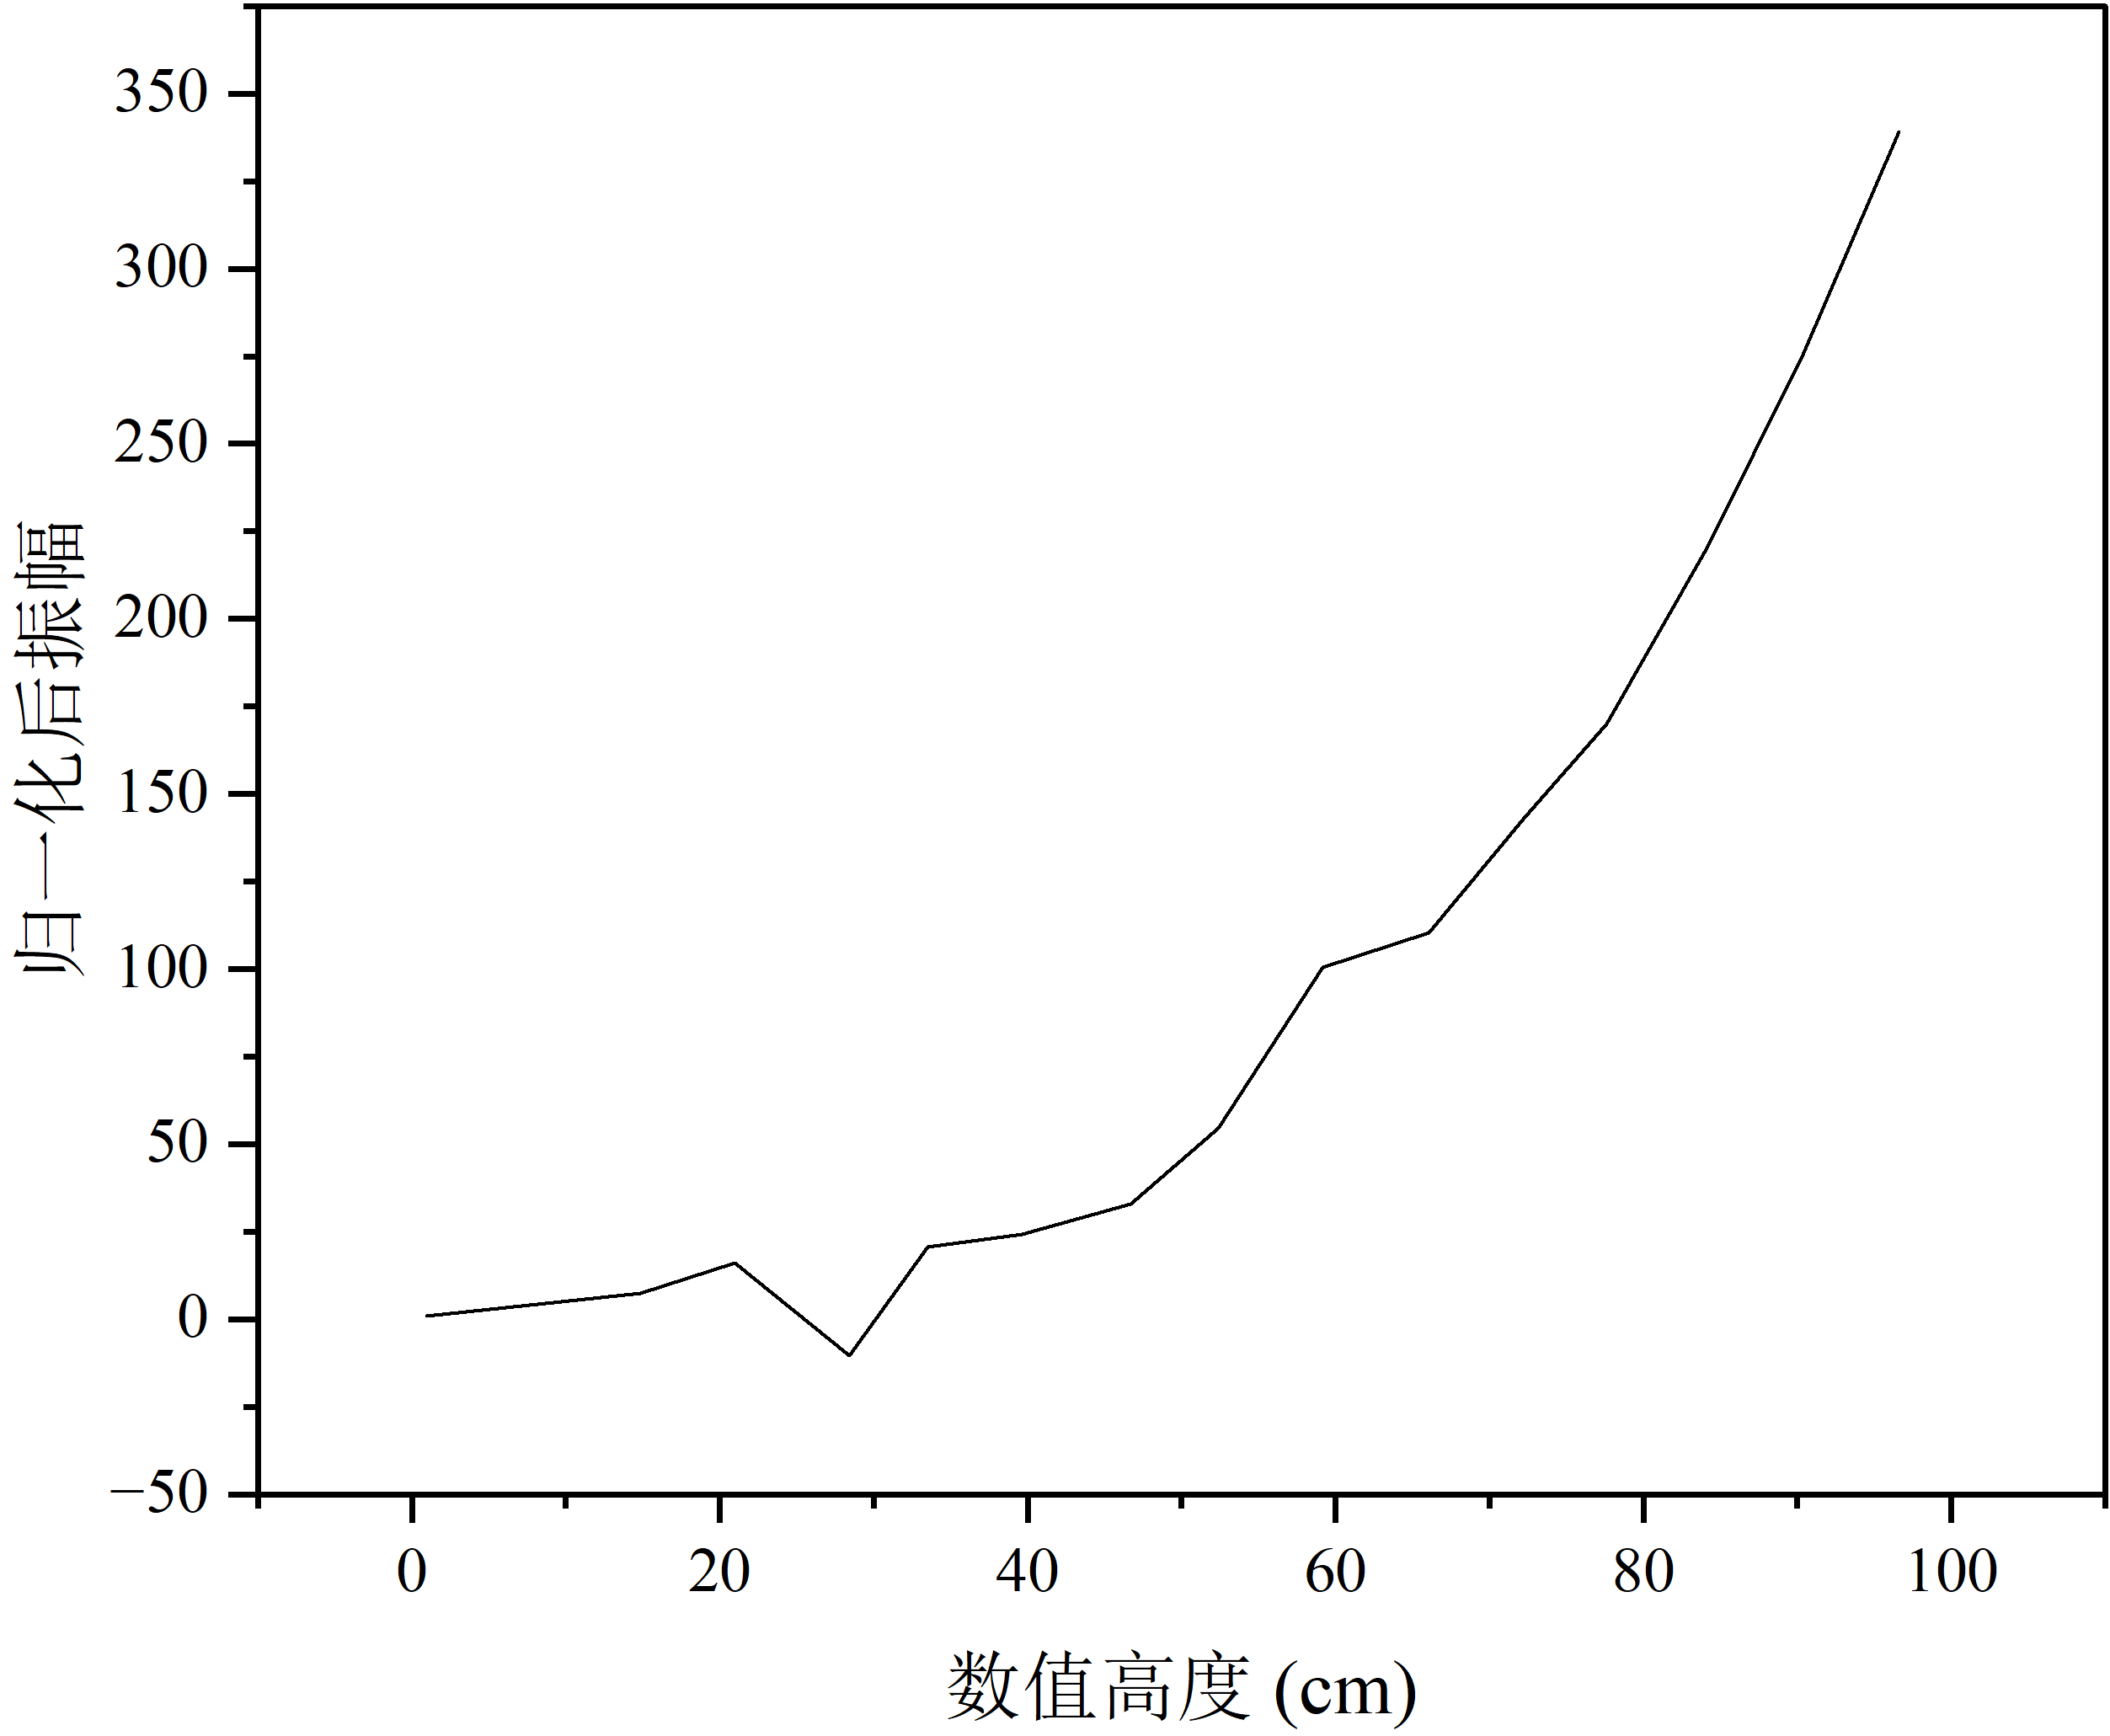
\includegraphics[width=\linewidth]{p10_img01.png}}\hfill
\subcaptionbox{二阶模态}[0.42\textwidth]{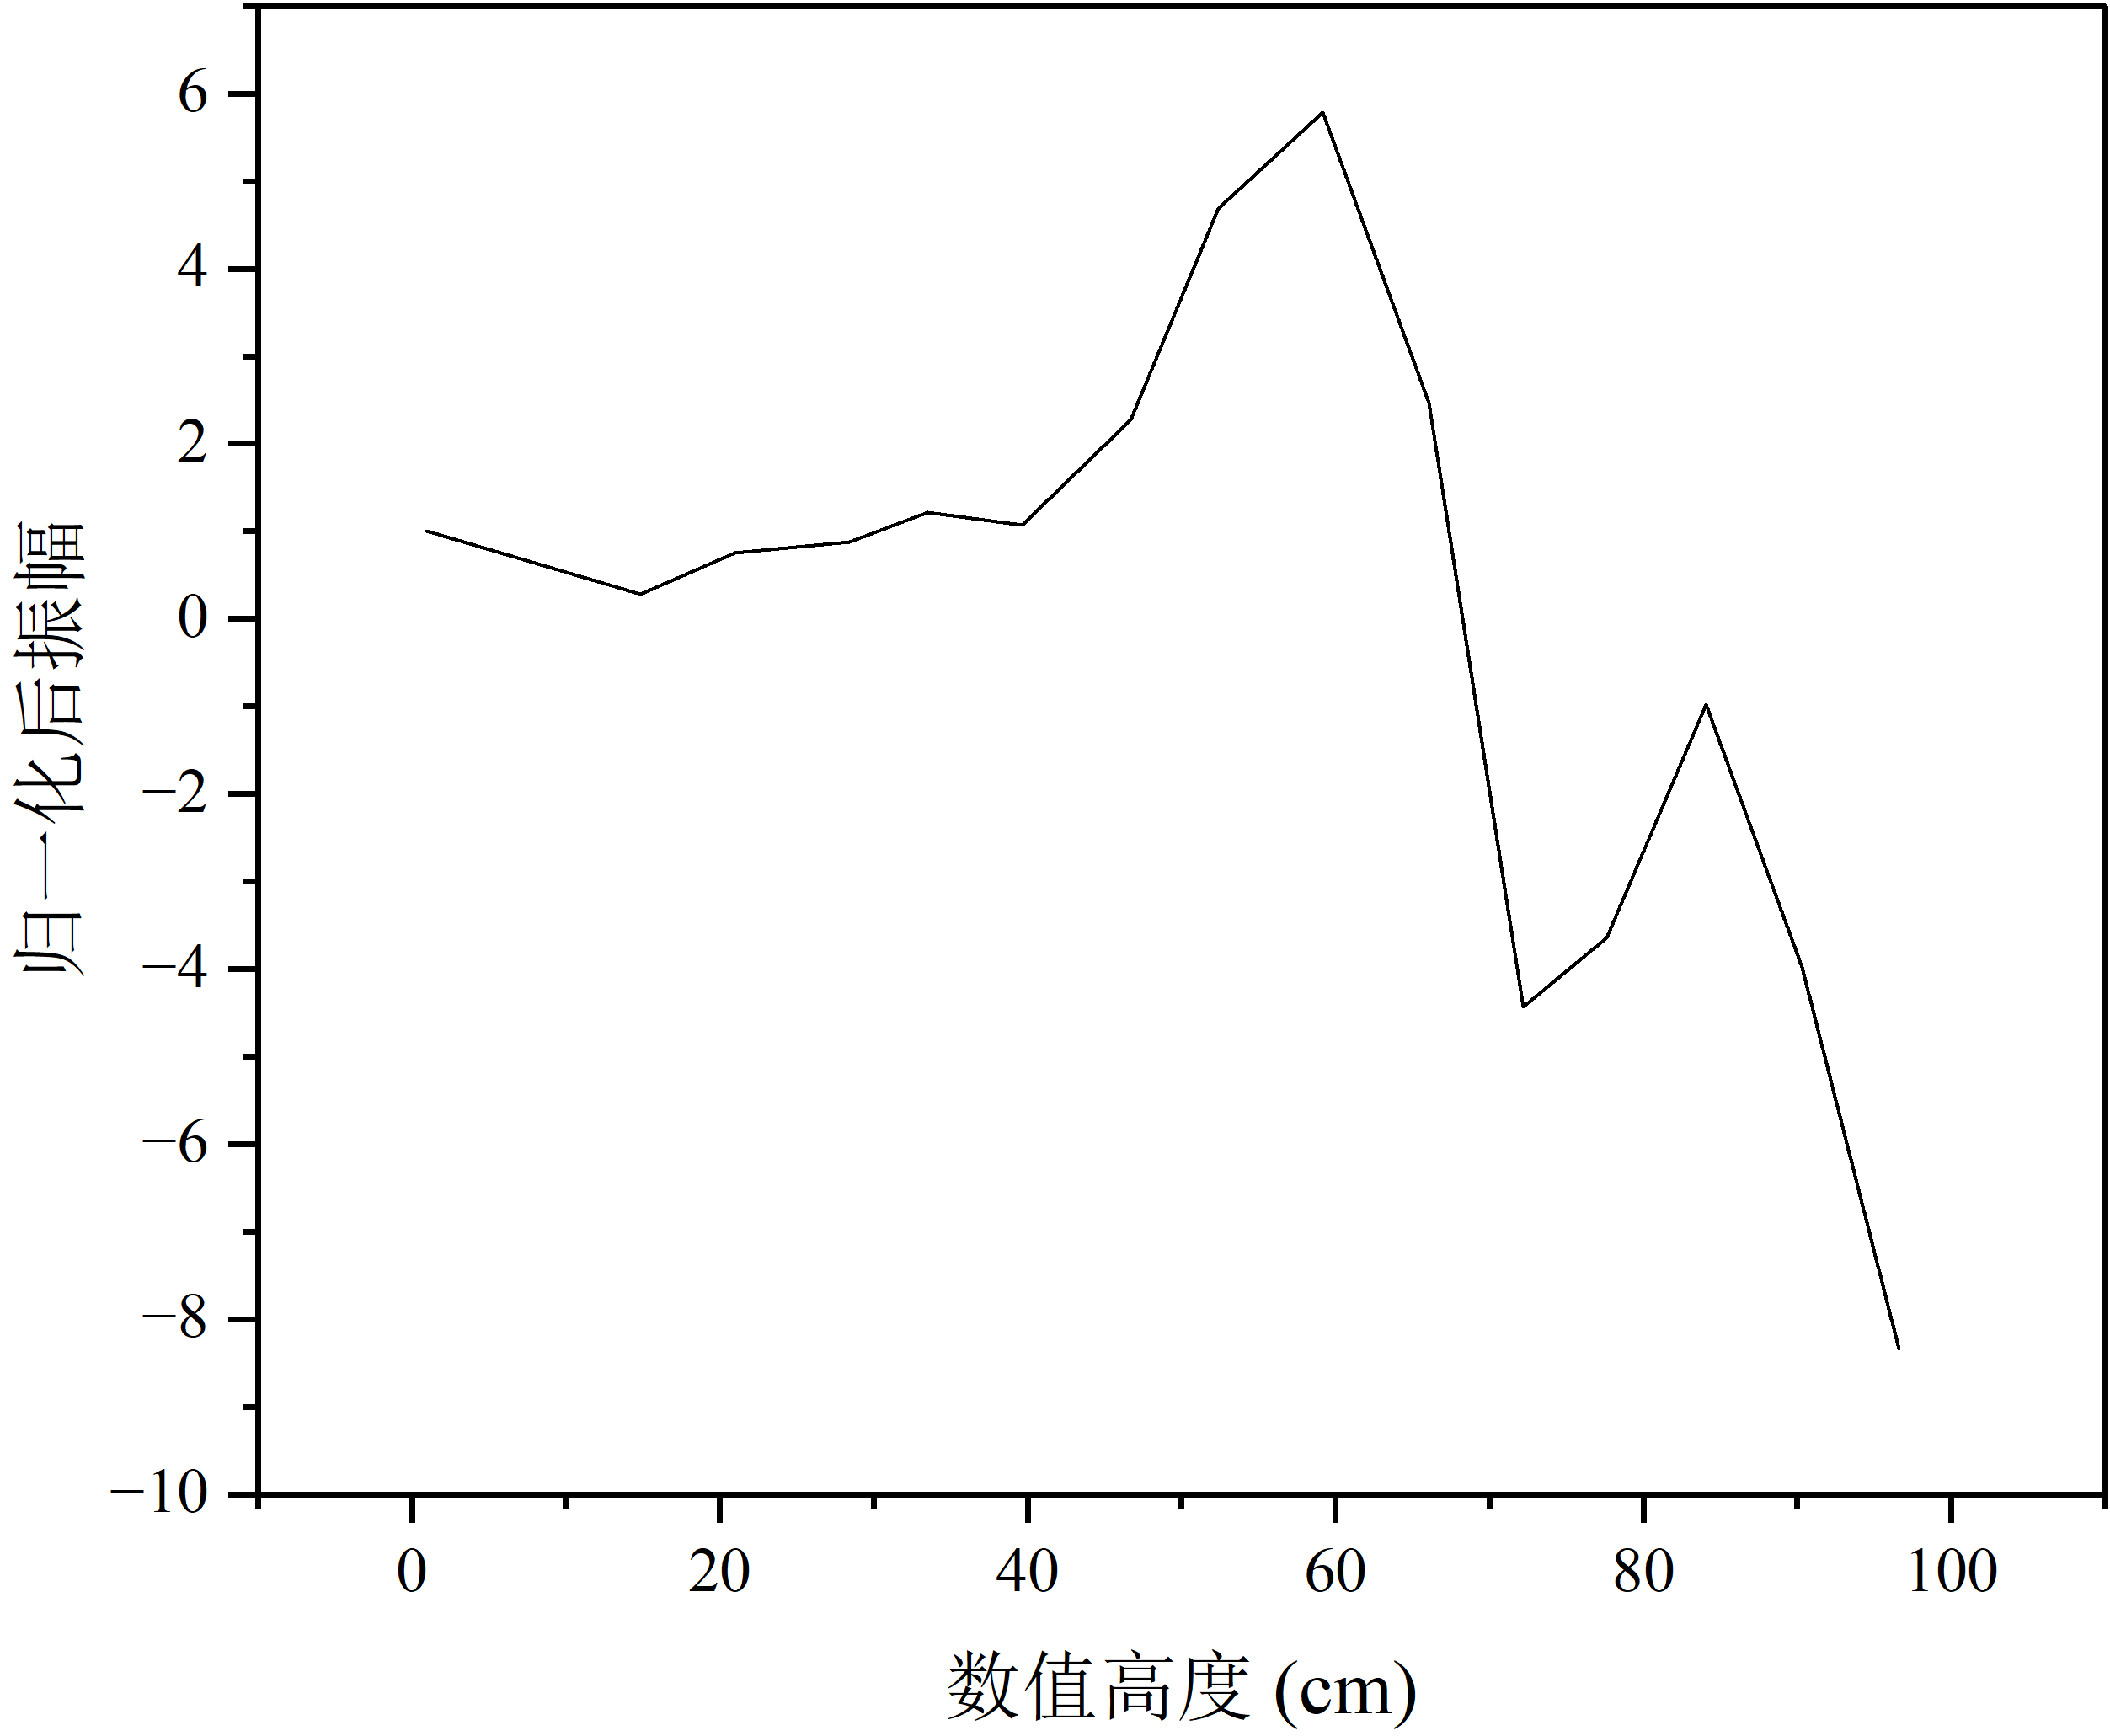
\includegraphics[width=\linewidth]{p10_img02.png}}\\[0.5em]
\subcaptionbox{三阶模态}[0.42\textwidth]{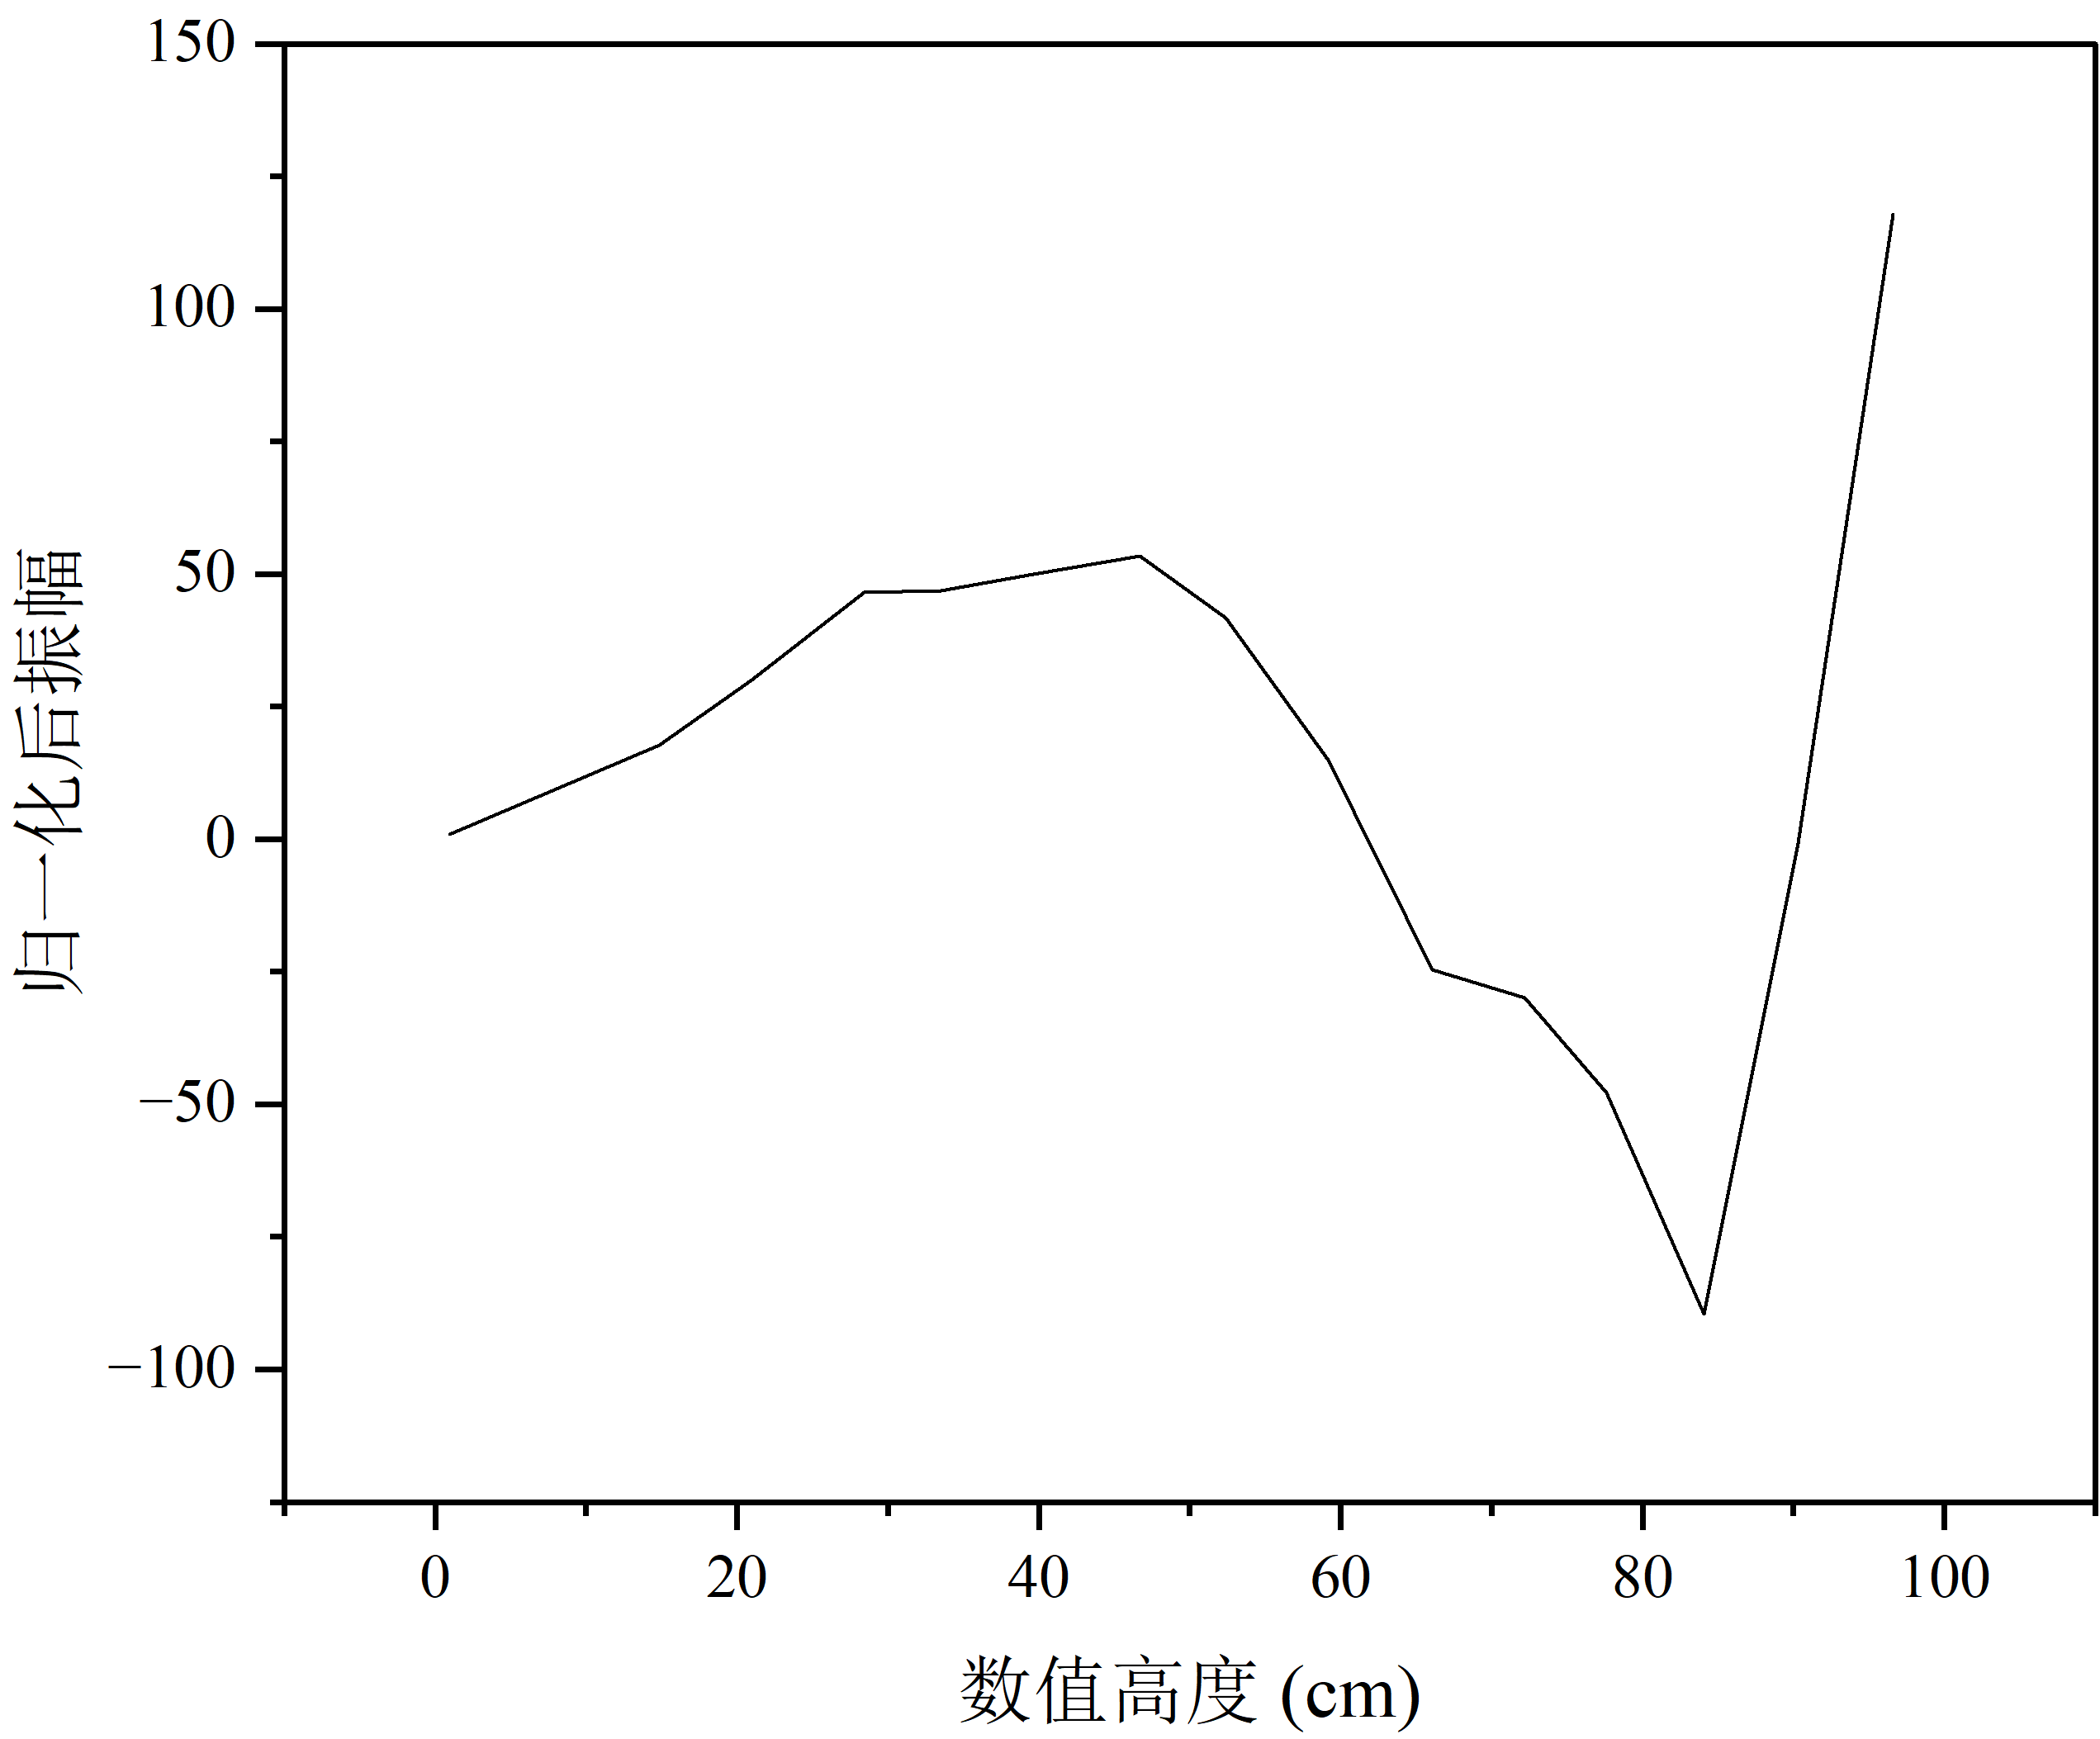
\includegraphics[width=\linewidth]{p10_img03.png}}\hfill
\subcaptionbox{四阶模态}[0.42\textwidth]{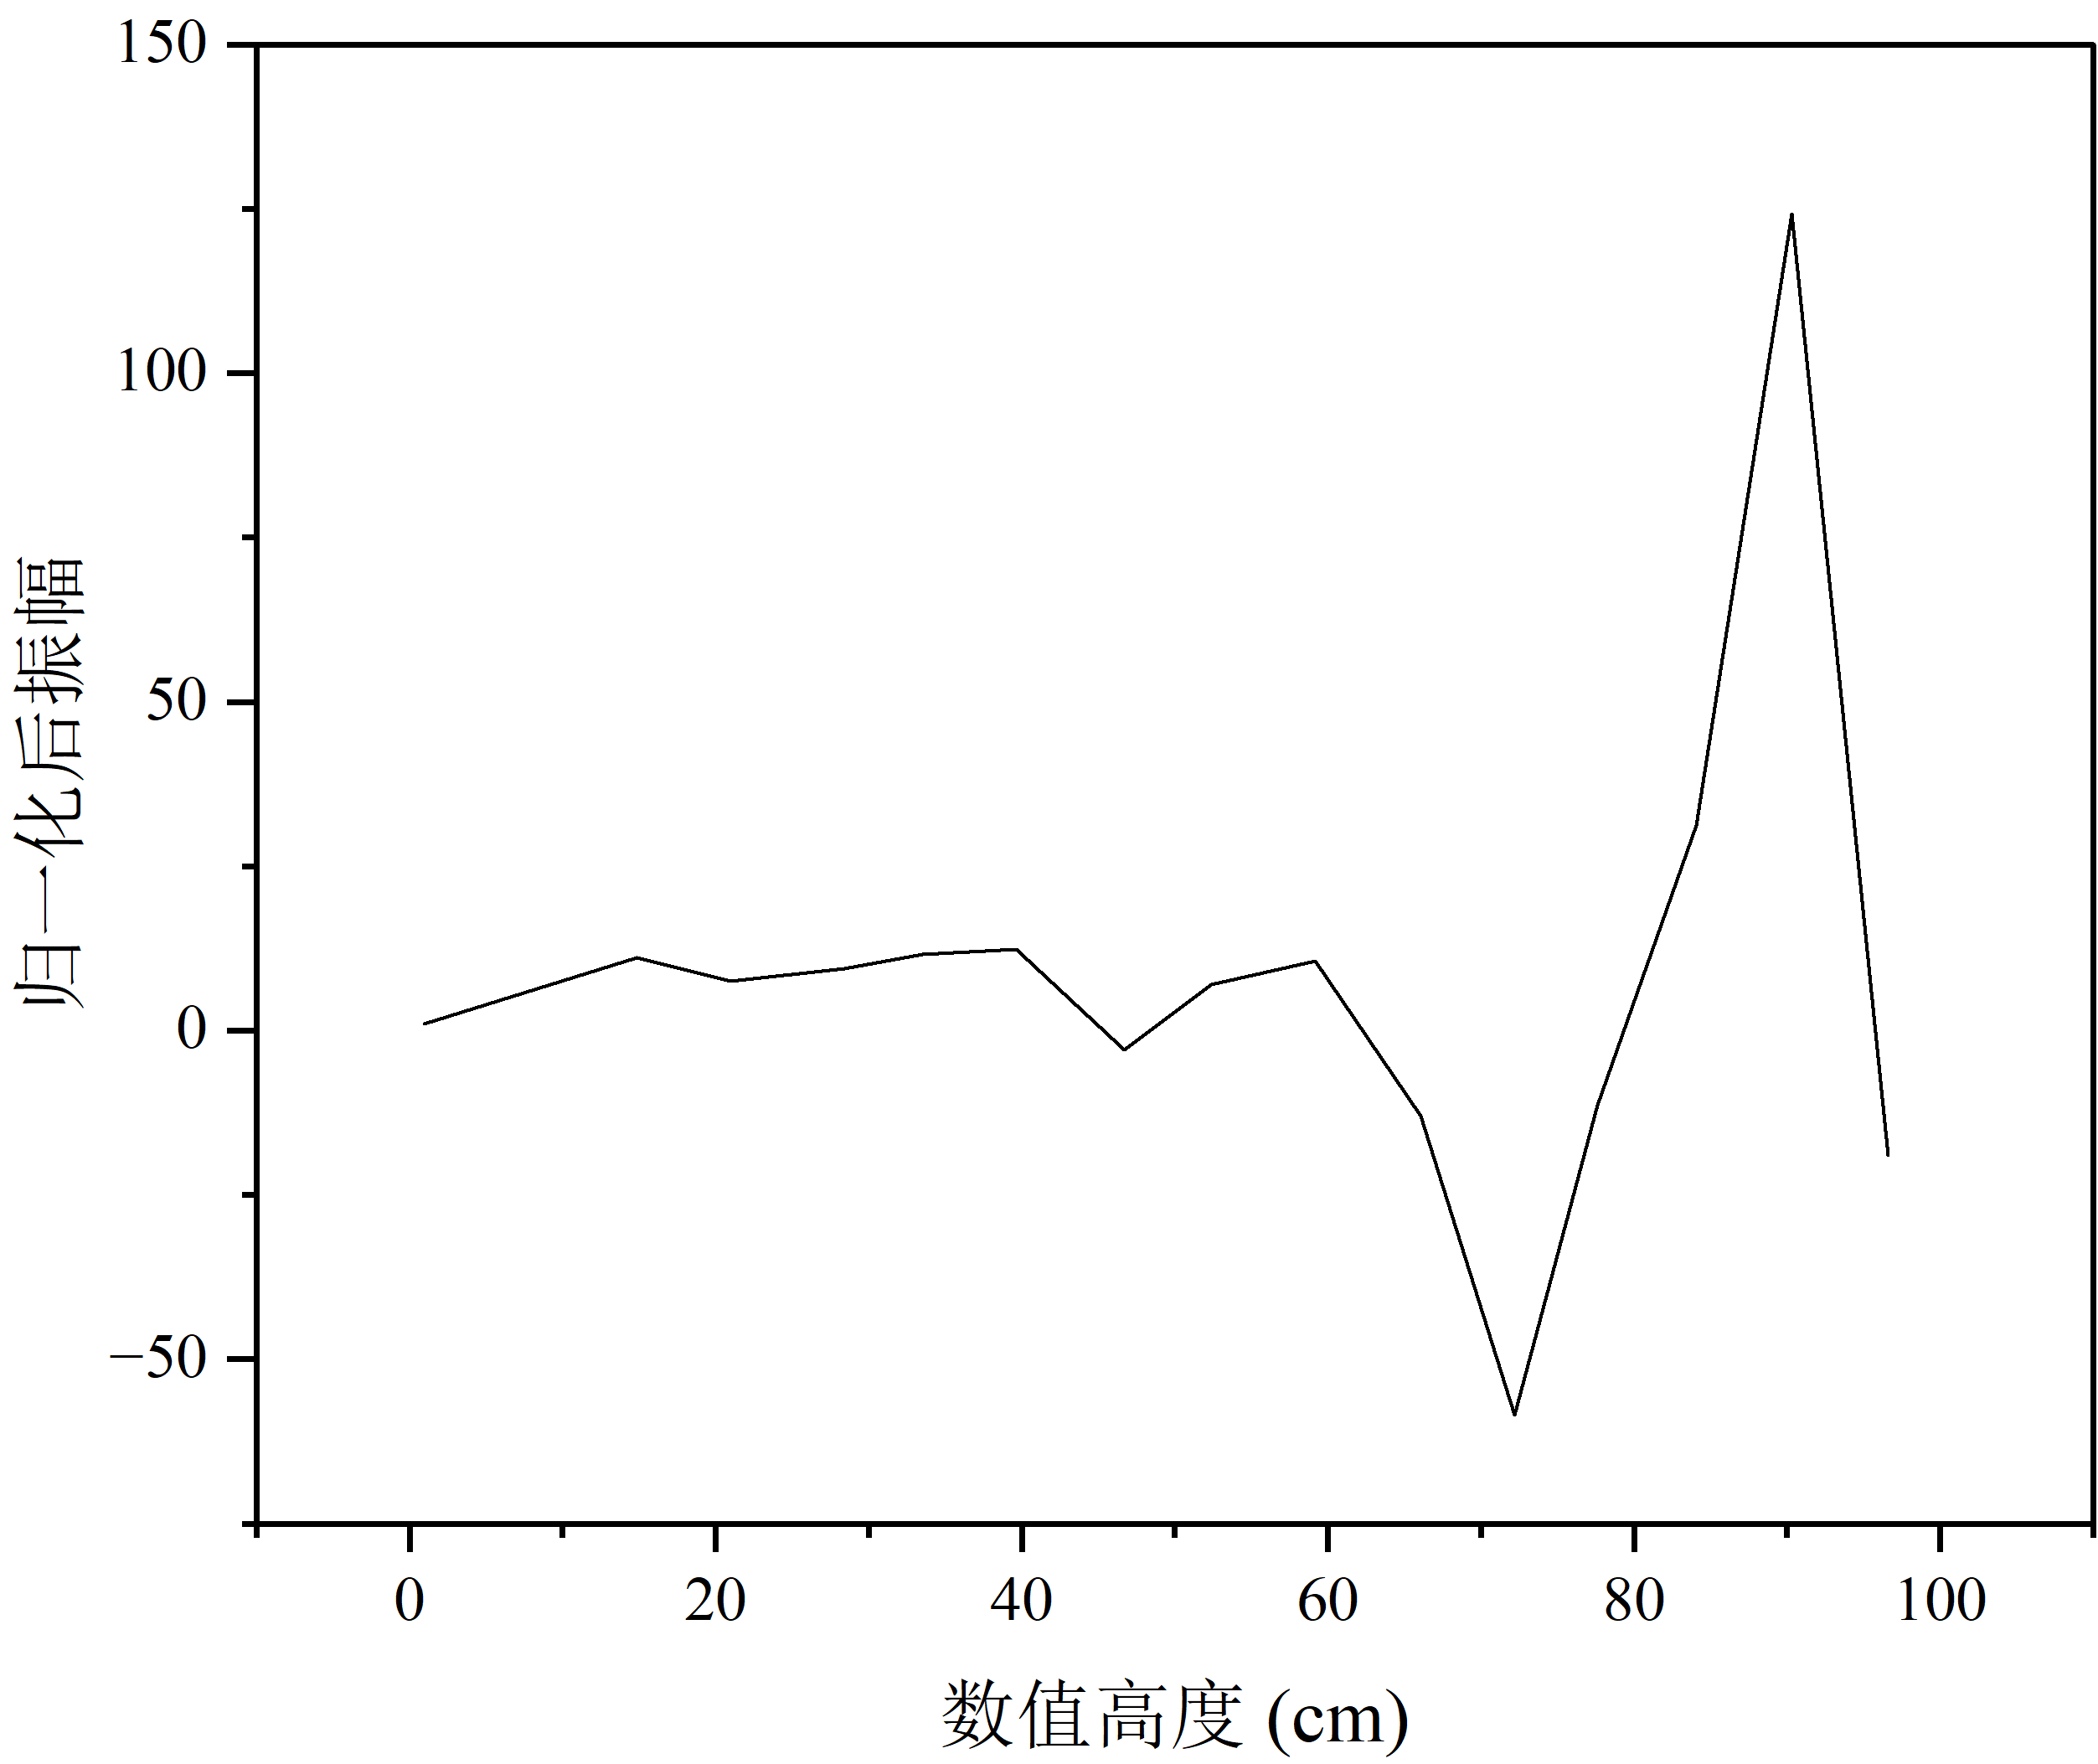
\includegraphics[width=\linewidth]{p10_img04.png}}\\[0.5em]
\subcaptionbox{五阶模态}[0.42\textwidth]{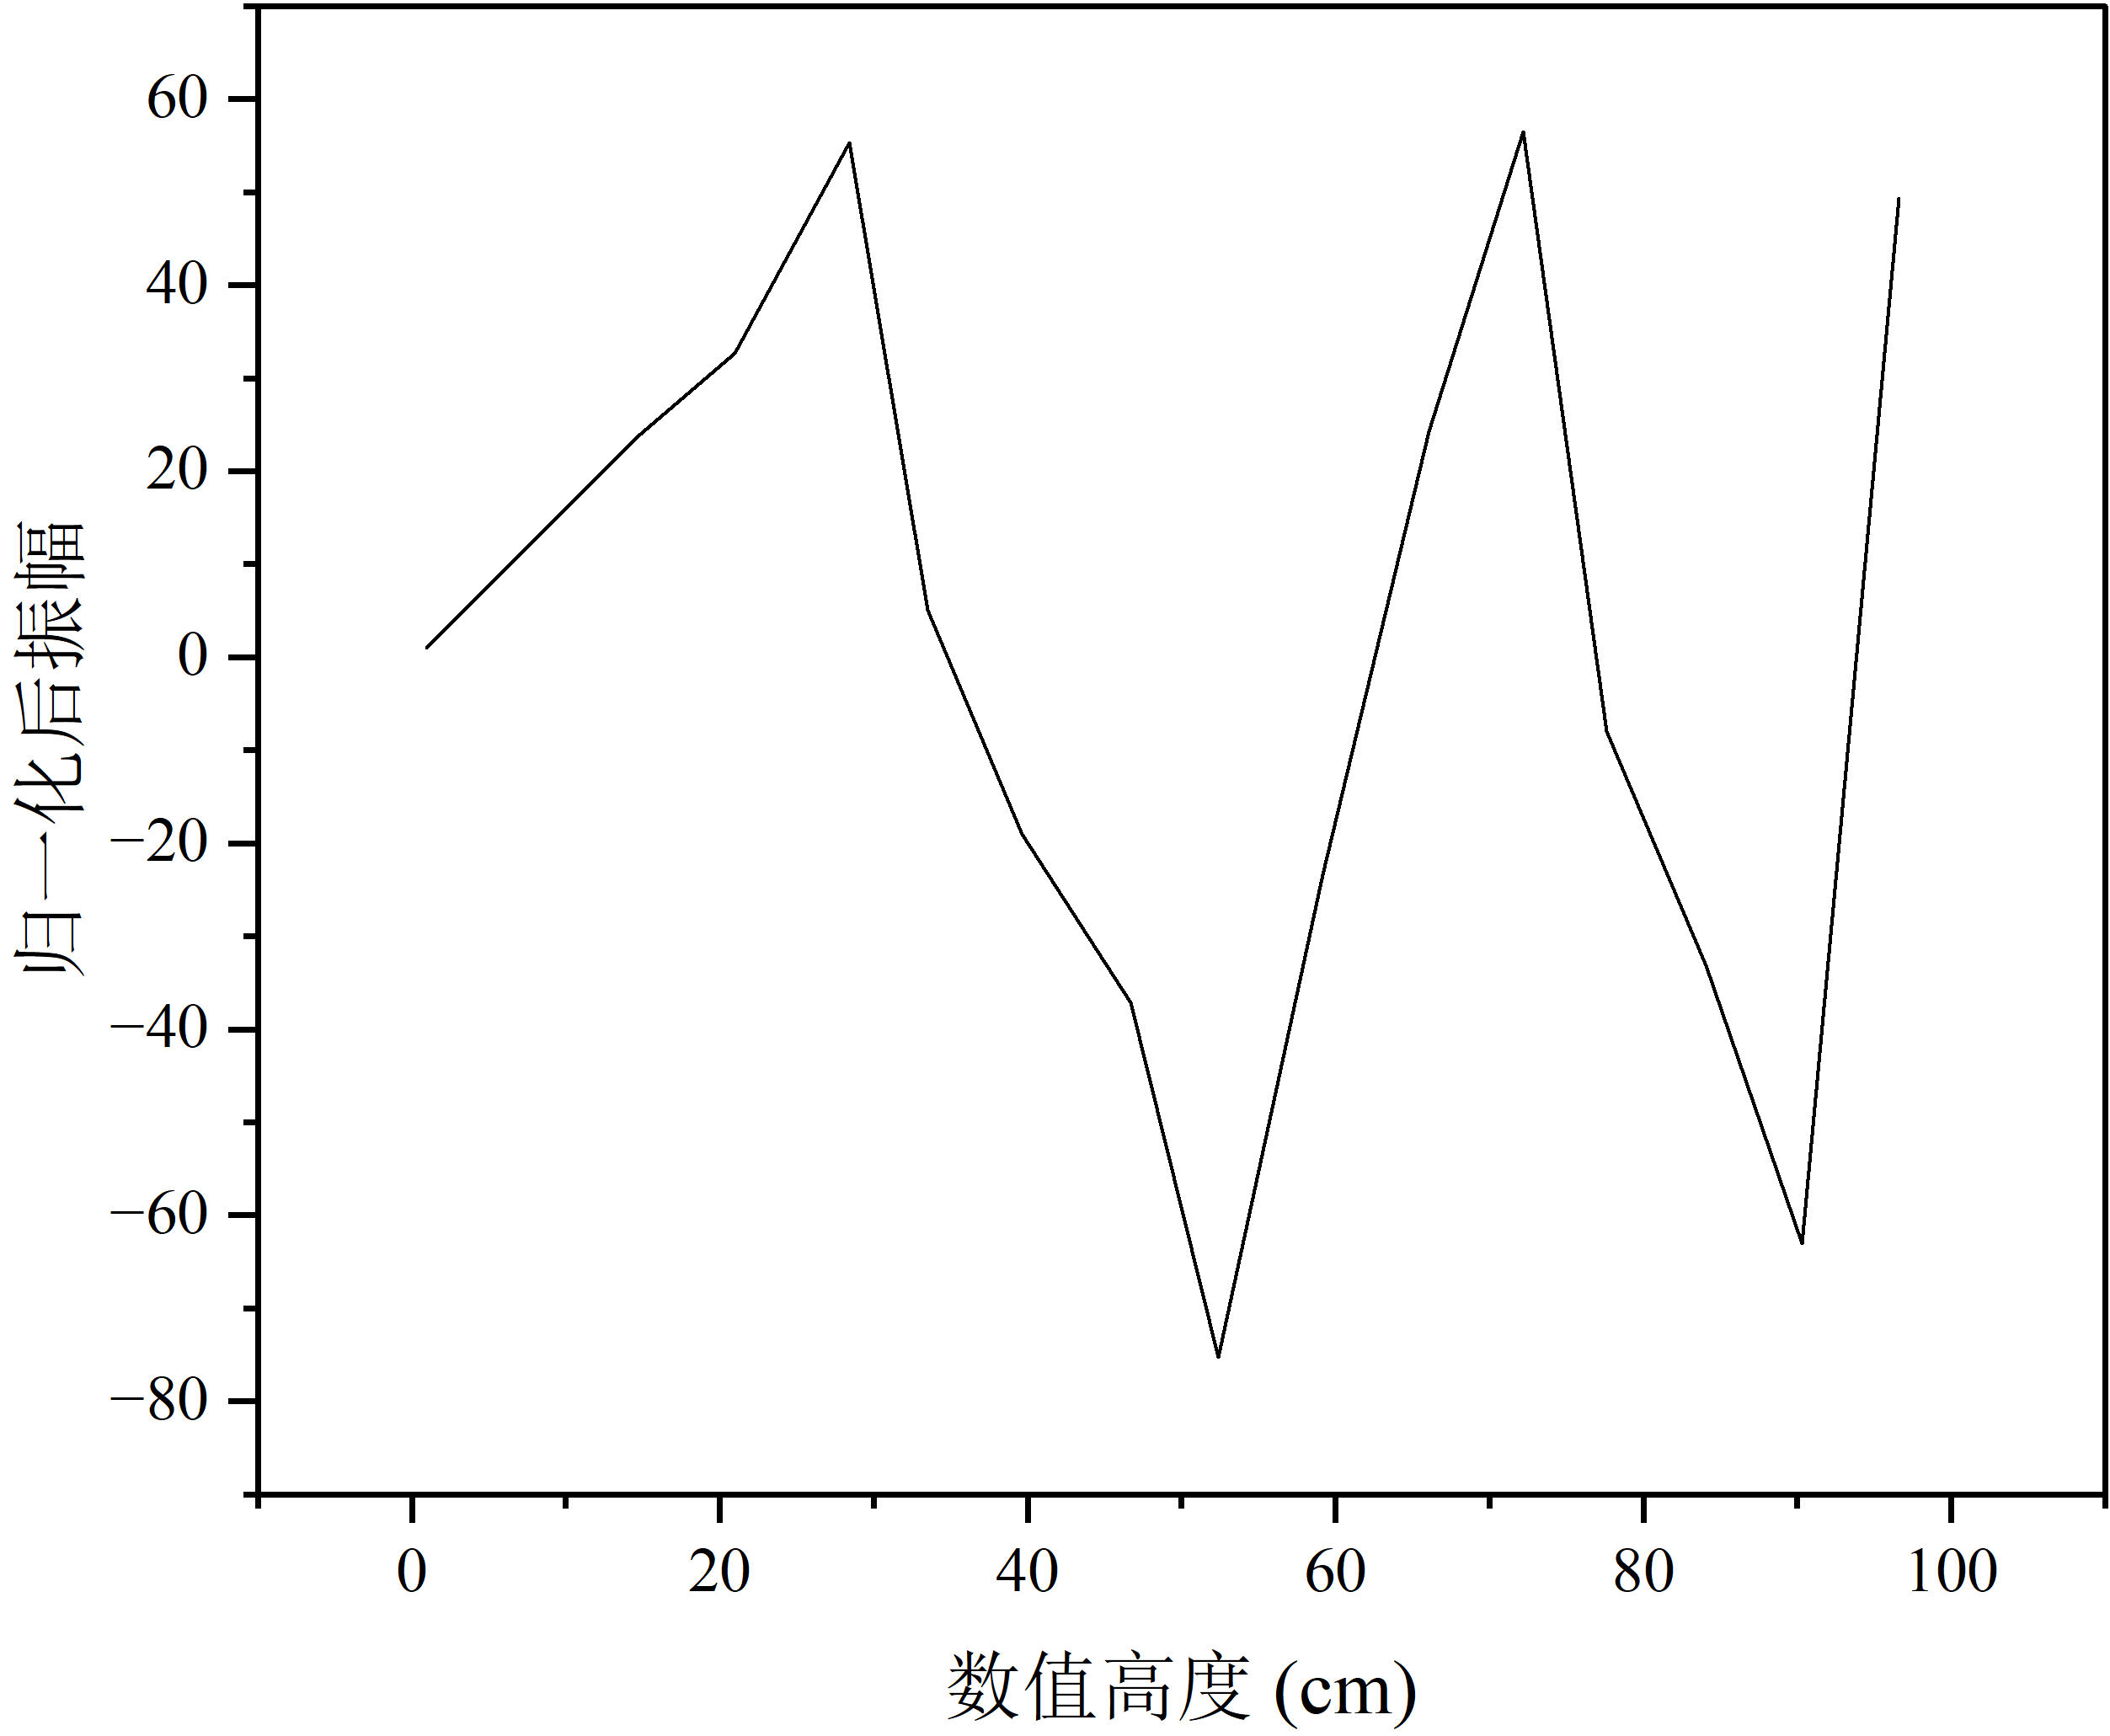
\includegraphics[width=\linewidth]{p10_img05.png}}
\caption{Pseudo Random 输入信号对应的前五阶固有模态}
\label{fig:exp5-random-modes}
\end{figure}

\section{结果分析与讨论}
分别使用周期线性调频脉冲激励信号（Periodic Chirp）和伪随机激励信号（Pseudo Random）测量叶片模型的固有频率、阻尼比以及振动模态。将实验得到的固有频率和阻尼比汇总于表\ref{tab:exp5-frequency-compare}和表\ref{tab:exp5-damping-compare}。

\begin{table}[H]
\centering\small
\caption{两种输入信号测得的叶片模型固有频率}
\label{tab:exp5-frequency-compare}
\begin{tabular}{lccccc}
\toprule
阶数 & 一阶 & 二阶 & 三阶 & 四阶 & 五阶\\
\midrule
Periodic Chirp 激励（Hz） & \blank[1.1cm] & \blank[1.1cm] & \blank[1.1cm] & \blank[1.1cm] & \blank[1.1cm]\\
Pseudo Random 激励（Hz） & \blank[1.1cm] & \blank[1.1cm] & \blank[1.1cm] & \blank[1.1cm] & \blank[1.1cm]\\
\bottomrule
\end{tabular}
\end{table}

\begin{table}[H]
\centering\small
\caption{两种输入信号测得的叶片模型阻尼率}
\label{tab:exp5-damping-compare}
\begin{tabular}{lccccc}
\toprule
阶数 & 一阶 & 二阶 & 三阶 & 四阶 & 五阶\\
\midrule
Periodic Chirp 激励 & \blank[1.1cm] & \blank[1.1cm] & \blank[1.1cm] & \blank[1.1cm] & \blank[1.1cm]\\
Pseudo Random 激励 & \blank[1.1cm] & \blank[1.1cm] & \blank[1.1cm] & \blank[1.1cm] & \blank[1.1cm]\\
\bottomrule
\end{tabular}
\end{table}

比较两种激励方式下测得的固有频率，说明固有频率是否受外部激励信号形式影响，并讨论不同实验环境下应如何选择激励方式。
\answer

分析所得到的模态振型是否符合前五阶模态特征，比较风力机叶片振型与悬臂梁振型的相似性，以及振型节点数与模态阶数的关系。
\answer

比较两种激励方式得到的阻尼比。分析实频曲线中的波动和毛刺对固有频率、半功率点识别及阻尼比计算的影响，并判断哪一组结果更可信、说明理由。
\answer

\section{误差分析}
\begin{enumerate}
  \item 由于激光发射器高度固定，在对竖直摆放的叶片模型进行测量时，不同测点之间可能因为激光发射器与模型表面之间角度的偏差而产生测量误差。
  \item 由于激励位置和叶片摆放的影响，实际模型中可能不仅存在弯曲振动，还可能激发扭转振动。这种振动模式的混合可能导致固有频率和半功率点识别出现偏差，从而影响实验结果的准确性。
  \item 本次实验选取的测量点数量为 15 个，相对较少。增加测量点数量可能有助于提高实验精度，从而获得更准确的模态参数。
  \item 风力机叶片本身并非完全对称，因此选择测量点时，左右位置的选取可能引入一定误差。
  \item 外界环境因素，如温度、湿度、振动等干扰，也可能影响实验测量结果。这些因素可能导致传感器性能波动，进而影响测量的准确性。
  \item 使用激光测振仪进行速度测量时，部分测量点的信号强度可能较低，尤其是在选择位置不当的情况下。这可能导致激光测振仪无法获得足够的反射信号，从而影响数据的准确性和可靠性。
\end{enumerate}
结合本组实验现象补充误差来源与改进措施。
\answer

\end{document}
